\documentclass{article}
% Global layout
\usepackage{fancyhdr, graphicx, hyperref, indentfirst, lastpage, setspace}

% Encoding
\usepackage[utf8]{vntex, inputenc}
\usepackage[english]{babel}
\usepackage{amsmath, amssymb, gensymb, textcomp}
%%%%%%%%%%%%%%%%%%%%%%%%%%%%%%%%%%%%%%%%%%%%%%%%%%%
\usepackage[utf8]{vietnam}
\usepackage{fontenc}
\usepackage{amsmath}
\usepackage{amsfonts}
\usepackage{amssymb}
\usepackage{graphics}
\usepackage{enumitem}
\usepackage{caption}
\usepackage{fancyhdr}
\usepackage[most]{tcolorbox}
\usepackage{mdframed}
\usepackage{fontawesome}
\usepackage{listings}
\usepackage{color}

\usepackage{setspace}

\usetikzlibrary{patterns}
\usetikzlibrary{calc,angles}

\definecolor{dkgreen}{rgb}{0,0.6,0}
\definecolor{gray}{rgb}{0.5,0.5,0.5}
\definecolor{mauve}{rgb}{0.58,0,0.82}
% Global layout
\usepackage%
[
        a4paper,
        % left=2cm,
        % right=2cm,
        % top=2cm,
        % bottom=2cm,
        % vmargin=2cm % vertical margins
        % hmargin=3cm % horizontal margins
        margin=3cm
]
{geometry}
\lstset{frame=tb,
  language=Java,
  aboveskip=3mm,
  belowskip=3mm,
  showstringspaces=false,
  columns=flexible,
  basicstyle={\small\ttfamily},
  numbers=none,
  numberstyle=\tiny\color{gray},
  keywordstyle=\color{blue},
  commentstyle=\color{dkgreen},
  stringstyle=\color{mauve},
  breaklines=true,
  breakatwhitespace=true,
  tabsize=3
}

\setcounter{tocdepth}{2}
% Encoding
\usepackage[utf8]{vntex, inputenc}
\usepackage[english]{babel}
\usepackage{amsmath, amssymb, gensymb, textcomp}
%%%%%%%%%%%% Bibliography %%%%%%%%%%%%
\usepackage[english]{babel}
\usepackage[backend=biber,style=alphabetic,sorting=ynt]{biblatex}
\usepackage{csquotes}

% Better table
\usepackage{array, booktabs, multicol, multirow, siunitx, tabularx}
% Wide tables go here https://tex.stackexchange.com/questions/332902/my-table-doesnt-fit-what-are-my-options
\usepackage{tcolorbox}
% Better enumerate
\usepackage{enumitem}

%%%%%%%%%%%% Code space %%%%%%%%%%%%
\usepackage[dvipsnames]{xcolor}
%\usepackage{tikz}

% Graphics
\usepackage{caption, float}

\usepackage{hyperref}

% Bibliography
\addbibresource{ref.bib} % references file
\nocite{*} % include all entries in references section

% Page setup
\allowdisplaybreaks{} % to have page breaks inside align* environment
\hypersetup{urlcolor=blue,linkcolor=black,citecolor=red,colorlinks=true}
\numberwithin{equation}{section}
\renewcommand{\arraystretch}{1.2} % space between table rows

% Global style setup
\makeatletter % change font size for not having underfull hbox
\renewcommand\Huge{\@setfontsize\Huge{22pt}{18}}
\makeatother

\AtBeginDocument{\renewcommand*\contentsname{Contents}}
\AtBeginDocument{\renewcommand*\refname{References}}
\setlength{\headheight}{40pt}

\pagestyle{fancy}
\fancyhead{} % clear all header fields
\fancyhead[L]{
  \begin{tabular}{rl}
    \begin{picture}(25,15)(0,0)
    \put(0,-8){
\includegraphics[width=8mm, height=8mm]{hcmut.png}}
    \end{picture}
    \begin{tabular}{l}
      \textbf{\bf \ttfamily University of Technology, Ho Chi Minh City}\\
      \textbf{\bf \ttfamily Faculty of Computer Science and Engineering}
    \end{tabular}
  \end{tabular}
}
\fancyhead[R]{
	\begin{tabular}{l}
		\tiny \bf \\
		\tiny \bf
	\end{tabular}  }
\fancyfoot{} % clear all footer fields
\fancyfoot[R]{\scriptsize \ttfamily Page {\thepage}/\pageref{LastPage}}
\renewcommand{\headrulewidth}{0.3pt}
\renewcommand{\footrulewidth}{0.3pt}
\newenvironment{code}[1]
{\VerbatimEnvironment%
  \begin{mdframed}[leftline=false,rightline=false,backgroundcolor=magenta!10,nobreak=false]%
    \begin{minted}[linenos=true,breaklines,breaksymbolleft=,obeytabs=true,tabsize=2]{#1}%
}
{
    \end{minted}%
  \end{mdframed}%
} % TODO Sample codeblock

\begin{document}

\begin{titlepage}
  \begin{center}
    VIETNAM NATIONAL UNIVERSITY, HO CHI MINH CITY \\
    UNIVERSITY OF TECHNOLOGY \\
    FACULTY OF COMPUTER SCIENCE AND ENGINEERING
  \end{center}

  \vspace{1cm}

  \begin{figure}[H]
    \centering
    
\includegraphics[width=0.5\textwidth]{hcmut.png}
  \end{figure}

  \vspace{1cm}

  \begin{center}
    \begin{tabular}{c}
      \textbf{\Large LẬP TRÌNH NÂNG CAO (CN-HK222)} \\
      {}                                             \\
      \midrule                                       \\
      \textbf{\Large Assignment (Semester 222)}          \\
      {}                                             \\
      \textbf{\Huge DESIGN PATTERN}         \\
      {}                                             \\
      \bottomrule
    \end{tabular}
  \end{center}

  \vspace{1cm}

  \begin{table}[h]
    \begin{tabular}{rll}
      \hspace{3cm} GVHD: & Mr.\ Trương Tuấn Anh &         \\
                            &                                  \\
      Students:             & Lê Nguyễn Phước Lộc & 2153544 \\
                            

    \end{tabular}
  \end{table}

  \begin{center}
    {\footnotesize HO CHI MINH CITY, MAY 2023} \\
  \end{center}
\end{titlepage}

%\thispagestyle{empty}

\tableofcontents

\newpage
\section{Giới Thiệu}
\subsection{Design Pattern là gì?}
\begin{itemize}
    \item Design Pattern là các giải pháp để xử lí với các vấn đề thông dụng khi lập trình OOP. Design Pattern như là những pattern được làm ra sẵn để lập trình viên có thể sử dụng dễ dàng để giải quyết vấn để ở trong đoạn code.
    \item Design Pattern giúp định hình cấu trúc và tương tác giữa các class trong hệ thống. Nó cung cấp một mô hình chuẩn để xây dựng các hệ thống có tính phân cấp, linh hoạt và dễ bảo trì. Mỗi Design Pattern mô tả một vấn đề cụ thể trong thiết kế phần mềm và cung cấp một giải pháp thích hợp cho vấn đề đó.
    \item Design Pattern không phải là một đoạn code cụ thể mà là một cách giải quyết cho vấn đề mà bạn xuất hiện. Patterns hay bị nhầm lẫn với Algorithms vì nó cùng là đoạn code để giải quyết vấn đề. Nhưng với Algorithms, nó là đoạn mã step by step thực hiện hành động còn Patterns là những chỉ dẫn nhưng nằm ở mức trừu tượng hơn. Một pattern khi sử dụng vào 2 chương trình khác nhau sẽ có code thực hiện khác nhau.
    \item Việc áp dụng Design Pattern trong thiết kế phần mềm giúp tăng tính linh hoạt, tái sử dụng và bảo trì của hệ thống, cũng như cung cấp một ngôn ngữ chung cho các nhà phát triển để truyền đạt ý tưởng và mô hình hóa thiết kế phần mềm.
\end{itemize}
\subsection{Tại sao ta nên học Design Pattern?}
\begin{itemize}
    \item Design Pattern thực tế là một công cụ hay giải pháp đã được kiểm nghiệm cho những vấn đề đơn giản trong lập trình. Thậm chí kể cả khi bạn không bao giờ gặp những vấn đề này trong thực tế thì việc học Design Pattern có thể giúp bạn hiểu rõ hơn các cấu trúc trong OOP.
    \item Design Pattern giúp xây dựng các phần mềm có tính linh hoạt cao và dễ dàng tái sử dụng. Thay vì phải xây dựng lại từ đầu, bạn có thể áp dụng các mẫu thiết kế đã tồn tại để tạo ra các thành phần phần mềm có tính cấu trúc và có thể tái sử dụng trong các dự án khác nhau.
    \item Nó cũng giúp các thành viên trong nhóm giao tiếp một cách dễ dàng hơn vì ta chỉ cần đưa ra thuật ngữ là các thành viên trong nhóm có thể dễ dàng hiểu được mà không cần phải giải thích chi tiết.
    \item Design Pattern giúp tăng hiệu suất phát triển phần mềm bằng cách cung cấp các mô hình đã được thử nghiệm và chứng minh. Thay vì phải xây dựng các giải pháp từ đầu, bạn có thể sử dụng Design Pattern để nhanh chóng triển khai các giải pháp đã được tối ưu hóa.
    \item Học Design Pattern giúp nâng cao kỹ năng thiết kế phần mềm của bạn. Bạn sẽ học cách phân tách các thành phần phần mềm, xác định các quy tắc tương tác giữa chúng và xây dựng cấu trúc phần mềm linh hoạt và mô-đun.
    \item Design Pattern được phát triển từ các kinh nghiệm thực tế của các nhà phát triển phần mềm. Bằng cách học Design Pattern, bạn có thể hưởng lợi từ sự giàu kinh nghiệm của người khác và áp dụng những kiến thức đã được chứng minh vào công việc của mình.
\end{itemize}

\subsection{Phân loại}
Design Pattern được phân loại dựa theo độ phức tạp (\textbf{Complexity}), mức độ chi tiết (\textbf{Level of detail}), và mức độ linh hoạt của Pattern cho tùy loại hệ thống (\textbf{Scale of applicability}).\\
Loại pattern được sử dụng rộng rãi là các Pattern kiến trúc (\textbf{Architectural Patterns}). Người sử dụng có thể implement các loại pattern này bằng nhiều ngôn ngữ khác nhau, nhưng trong bài báo cáo này ta chủ yếu sử dụng ngôn ngữ \textbf{C++} để dễ hình dung và quen thuộc. Các pattern còn có thể được sử dụng để thiết kế toàn bộ hệ thống.\\
Các pattern còn được phân loại dựa theo mục đích sử dụng. Ở bài báo cáo này, chủ yếu 3 loại Patterns sẽ được đề cập.\\
\begin{itemize}
    \item \textbf{Creational Patterns}: là pattern cung cấp một cơ chế tạo ra các đối tượng với tính linh hoạt cao và dễ sử dụng lại.
    \item \textbf{Structural Patterns}: là pattern cung cấp cơ chế liên kết các classes với nhau thành cấu trúc lớn hơn và linh hoạt, dễ sử dụng hơn.
    \item \textbf{Behavioral Patterns}: là pattern dùng để thực hiện hành vi của các đối tượng đồng thời là sự giao tiếp của các đối tượng với nhau.
\end{itemize}
\begin{center}
  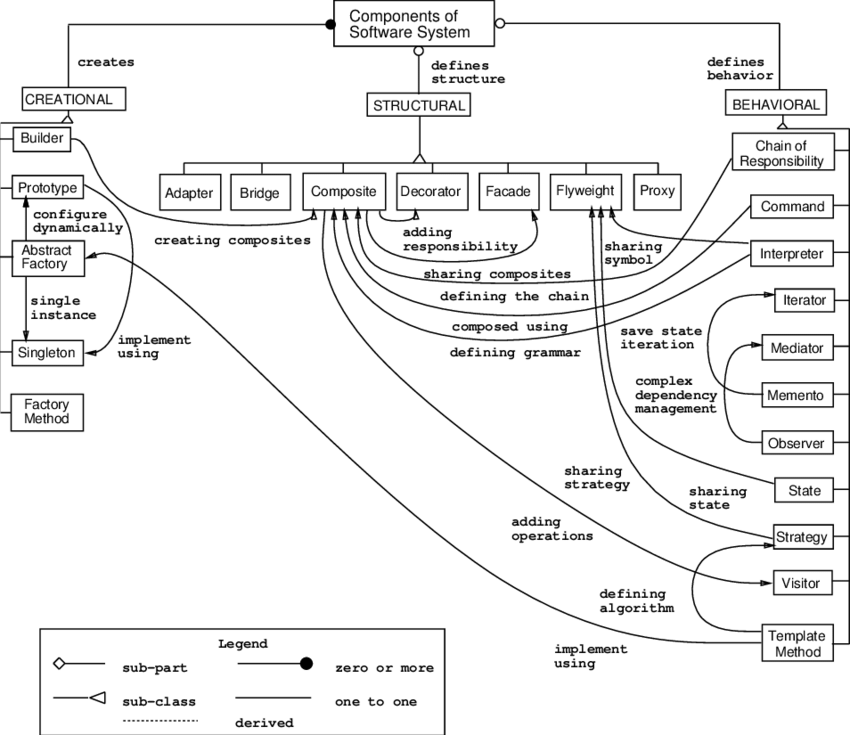
\includegraphics[scale=0.5]{image/dp3.png}  
\end{center}
Phía trên là sơ bộ các mối quan hệ giữa các Patterns với nhau. Có thể dễ dàng thấy các Patterns này đếu được phát triển tử các Pattern khác, nên trong tương lai có khả năng sẽ có thể xuất hiện thêm nhiều Pattern tiện lợi và hiện đại hơn.

\newpage
\section{Creational Patterns}
Ở phần Creational Patterns, ta có 5 mẫu Patterns cụ thể là \textbf{Factory Method}, \textbf{Abstract Factoy Method}, \textbf{Builder}, \textbf{Prototype}, \textbf{Singleton}. Nhờ vào 5 mẫu này mà ta có thể tạo ra các objects mà vẫn che giấu được logic để tạo ra nó thay vì tạo một cách trực tiếp.\\
\subsection{Factory Method}
\subsubsection{Địng nghĩa}
Factory Method là một Pattern dùng để cung cấp interface để tạo các objects ở trong super-class, nhưng cho phép các sub-classes quyết định xem loại object nào sẽ được tạo ra.
\subsubsection{Cách sử dụng}
Ta sử dụng factory method trong các trường hợp sau:
\begin{itemize}
    \item Khi bạn muốn tạo một Object mà không cần xác định Object đó thuộc Class nào. Thay vì tạo Object bằng cách gọi trực tiếp từ constructor, bạn sẽ sử dụng một phương thức factory để tạo đối tượng.
    \item Khi bạn muốn có một hệ thống dễ dàng mở rộng bởi vì Factory Method cho phép bạn mở rộng việc tạo các Object bằng cách thêm các SubClass mới mà không làm thay đổi mã nguồn của SuperClass.
    \item Khi bạn muốn áp dụng các kỹ thuật khác nhau để tạo ra Object dựa trên các yêu cầu hoặc tình huống khác nhau. Factory Method cho phép bạn triển khai các phương thức factory khác nhau trong các SubClass để tạo đối tượng theo cách tùy chỉnh.
\end{itemize}
\subsubsection{Cấu trúc}
Factory Method Pattern gợi ý chúng ta thay vì sử dụng phương thức gọi trực tiếp (\textbf{new} operator), chúng ta gọi thông qua một hàm của factory và các hàm này thường trả về loại object. Các thành phần chính của mẫu: \\
\begin{itemize}
    \item Một interface định nghĩa khuôn mẫu cho các sản phẩm được tạo ra.
    \item Các subclass kế thừa từ interface tạo ra hàng loạt loại sản phẩm khác nhau.
    \item Một interface định nghĩa factory method trả về kiểu đối tượng sản phẩm.
    \item Các subclass kế thừa từ interface trên tạo ra hàng loạt class trả về các đối tượng sản phẩm cần.
\end{itemize}
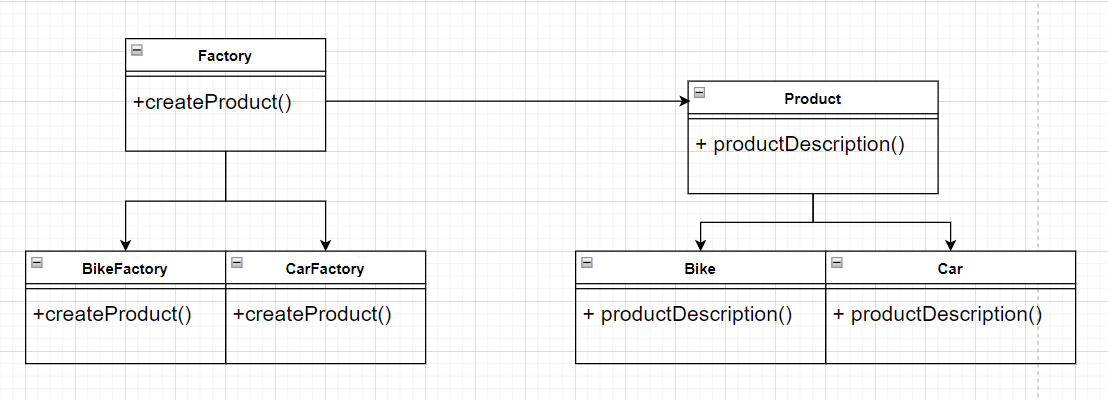
\includegraphics[scale=0.65]{image/creational/cso.png}
\subsubsection{Ưu điểm và Nhược điểm}
Ta thường thấy các ưu nhược điểm sau:\\\\
Ưu điểm:
\begin{itemize}
    \item Tăng tính linh hoạt và tái sử dụng trên nhiều dự án khác nhau, nhiều ngôn ngữ khác nhau.
    \item Dễ dàng mở rộng hay thu hẹp quy mô dự án mà không ảnh hưởng đến các bộ phận khác do các Class khởi tạo không liên quan trực tiếp với nhau.
\end{itemize}
Nhược điểm:
\begin{itemize}
    \item Tăng độ phức tạp: Factory Method có thể làm tăng độ phức tạp của mã nguồn, đặc biệt là khi có nhiều lớp con và các phương thức factory tương ứng.
    \item Nếu không được sử dụng đúng cách, Factory Method có thể dẫn đến việc tạo ra nhiều SubClass thừa thãi không cần thiết.
    \item Khó khăn trong việc theo dõi luồng tạo Object: Khi sử dụng Factory Method, việc theo dõi và hiểu rõ luồng tạo đối tượng có thể trở nên phức tạp khi hệ thống có nhiều SubClass.
\end{itemize}
\subsubsection{Code Example}
Sau đây là code ví dụ mẫu cho Factory Method Pattern có 2 sản phẩm là Bike và Car, cùng với 2 loại Factory là bikeFactory và carFactory. \\
\begin{lstlisting}
#include <iostream>
using namespace std;

class Product
{
public:
    virtual void productDescription() = 0;
};

class Bike : public Product
{
public:
    void productDescription() override { cout << "Bike" << endl; }
};

class Car : public Product
{
public:
    void productDescription() override { cout << "Car" << endl; }
};
//--------------------Factory---------------------
class Factory
{
public:
    virtual Product *createProduct(int n = 0) = 0;
};

class bikeFactory : public Factory
{
public:
    Product *createProduct(int a) override { return new Bike; }
};

class carFactory : public Factory
{
public:
    Product *createProduct(int a) override { return new Car; }
};

int main()
{
    Factory *factory = new bikeFactory();
    factory->createProduct()->productDescription();
    Factory *factory2 = new carFactory();
    factory2->createProduct()->productDescription();
}
\end{lstlisting}
Ở hàm main(), ta tạo 2 nhà máy để sản xuất 2 loại xe khác nhau và cho in ra thông tin 2 loại xe đó.\\
\newline
\textbf{Kết quả:}
\begin{lstlisting}
Bike
Car
\end{lstlisting}
\subsubsection{Các Pattern liên quan}
\begin{itemize}
    \item Thông thường, Factory method hay được sử dụng chung với Abstract Factory Method.
    \item Prototypes: trong một số trường hợp không yêu cầu phân lớp từ Creator. Tu nhiên, chúng thường khởi tạo trên các lớp product.
\end{itemize}
\subsection{Abstract Factory Method}
\subsubsection{Định nghĩa}
Abstract Factory Method là một Pattern dùng để tạo ra tập hợp các objects liên quan với nhau mà không cần phải làm rõ các class thành phần.
\subsubsection{Cách sử dụng}
Ta thông thường sử dụng Abtract Factory Method trong các trườn g hợp sau:
\begin{itemize}
    \item 1. Bạn muốn tạo ra một nhóm các Object có liên quan với nhau, hỗ trợ một loạt chức năng liên quan.
    2. Bạn muốn đảm bảo rằng các Objet được tạo ra phù hợp với nhau và tuân thủ các quy tắc nhất định.
    \item 3. Bạn muốn ẩn thông tin về cách tạo ra các Object cụ thể và chỉ tương tác thông qua giao diện chung.
\end{itemize}
\subsubsection{Cấu trúc}
Đầu tiên, ta cần gom tất cả các sản phẩm chung loại vào một lớp interface. Sau đó, ta cần tạo ra một Abstract Factory có chứa toàn bộ các phương thức để tạo ra các loại sản phẩm khác nhau.\\
Với mỗi sản phẩm trong cùng 1 loại, ta tạo ra các Factory cho riêng nó chứa các phương thức để tạo ra các kiểu sản phẩm của loại sản phẩm đó.\\
\newline
\begin{center}
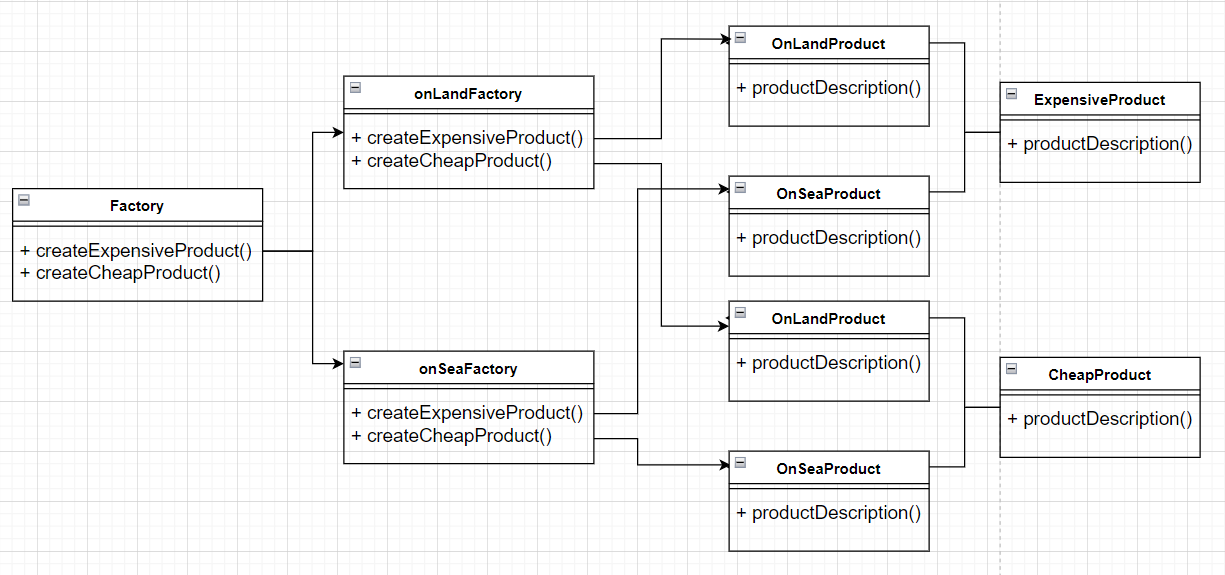
\includegraphics[scale=0.60]{image/creational/afso.png}
\end{center}
Các thành phần chính trong mô hình:
\begin{itemize}
    \item Một interface hoặc abstract class chứa các phương thức để tạo ra các đối tượng sản phẩm.
    \item Các class kế thừa từ interface có nhiệm vụ cài đặt, thực hiện các phương thức tạo nên sản phẩm. Mỗi một class tương ứng chỉ tạo ra duy nhất một loại sản phẩm.
    \item Một interface hoặc abstract class cho một tập hợp các loại sản phẩm liên quan với nhau.
    \item Một loạt các loại sản phẩm liên quan đến nhau kế thừa từ class interface trên.
\end{itemize}
\subsubsection{Ưu điểm và Nhược điểm}
Ta thường thấy một số ưu nhược điểm như sau:\\\\
Ưu điểm:
\begin{itemize}
    \item Nhìn chung Abtract Factory Method hoàn toàn giống với Factory Method ngoài độ ứng dụng với các chương trình lớn ra.
\end{itemize}
Nhược điểm:
\begin{itemize}
    \item Sử dụng Abstract Factory method yêu cầu bạn xây dựng các lớp Factory và Concrete Factory cụ thể. Điều này có thể tạo ra sự phụ thuộc cao giữa các lớp và làm cho mã khó hiểu hơn nếu không được sử dụng một cách hợp lý.
    \item Việc tạo ra các đối tượng thông qua Abstract Factory có thể tạo ra tiềm ẩn lỗi nếu không xử lý tốt việc tạo đối tượng.
\end{itemize}
\subsubsection{Code}
\begin{itemize}
    \item Chúng ta có 2 loại sản phẩm là sản phẩm đắt tiền và sản phẩm rẻ hơn.
    \item Ở sản phẩm đắt, ta có 2 loại là Xe hơi và Du thuyền. Còn đối với loại sản phẩm rẻ tiền hơn, ta có Xe đạp và Thuyền.
    \item Ta có 2 loại nhà máy là nhà máy sản xuất các phương tiện trên bờ và nhà máy sản xuất các phương tiện trên mặt nước.
\end{itemize}

\begin{lstlisting}
#include <iostream>
using namespace std;

//--------------------------------------
class ExpensiveProduct
{
public:
    virtual void productDescription() = 0;
};

class CheapProduct
{
public:
    virtual void productDescription() = 0;
};
//--------------------------------------
class Bike : public CheapProduct
{
public:
    void productDescription() override { cout << "Bike" << endl; }
};

class Boat : public CheapProduct
{
public:
    void productDescription() override { cout << "Boat" << endl; }
};

class Car : public ExpensiveProduct
{
public:
    void productDescription() override { cout << "Car" << endl; }
};

class Yatch : public ExpensiveProduct
{
public:
    void productDescription() override { cout << "Yatch" << endl; }
};
//--------------------Factory---------------------
class Factory
{
public:
    virtual CheapProduct *createCheapProduct() = 0;
    virtual ExpensiveProduct *createExpensiveProduct() = 0;
};
//------------------------------------------------
class onLandFactory : public Factory
{
public:
    ExpensiveProduct *createExpensiveProduct() override { return new Car; };
    CheapProduct *createCheapProduct() override { return new Bike; };
};

class onSeaFactory : public Factory
{
public:
    ExpensiveProduct *createExpensiveProduct() override { return new Yatch; };
    CheapProduct *createCheapProduct() override { return new Boat; };
};
//-----------------------------------------------

int main()
{
    Factory *f1 = new onLandFactory();
    f1->createCheapProduct()->productDescription();
    f1->createExpensiveProduct()->productDescription();
    Factory *f2 = new onSeaFactory();
    f2->createCheapProduct()->productDescription();
    f2->createExpensiveProduct()->productDescription();
}
\end{lstlisting}
Ở hàm main, ta tạo ra nhà máy sản xuất phương tiện di chuyển trên mặt đất rồi sản xuất lần lượt các sản phẩm đắt tiền và rẻ tiền, tương tự với nhà máy sản xuất phương tiện di chuyển trên mặt nước.\\
\newline
\textbf{Kết quả:}
\begin{lstlisting}
Bike
Car
Boat
Yatch
\end{lstlisting}
\subsubsection{Các Pattern liên quan}
\begin{itemize}
    \item Factory Method: đây là nguồn gốc để phát triển lên được Abstract Factory.
    \item Builder: có thể kết hợp với Builder để chạy một vài bước tạo sản phẩm trước khi Abstract Factory trả về sản phẩm.
    \item Prototype: đương nhiên việc mỗi class khởi tạo của Abstract Factory có thêm một hàm clone() cũng không phải việc gì quá khó khăn.
    \item Singleton: hoặc là ta có thể làm cho các đối tượng mà Abstract Factory tạo là là duy nhất và được truy cập từ khắp nơi trên mã nguồn.
\end{itemize}

\subsection{Builder}
\subsubsection{Định nghĩa}
Builder Pattern cũng là một loại Creational Pattern cho phép bạn xây dựng các đối tượng phức tạp từng bước.
\subsubsection{Cách sử dụng}
Thông thường, ta sẽ sử dụng Builder trong các trường hợp sau:
\begin{itemize}
    \item Bạn muốn xây dựng một Object phức tạp bằng cách kết hợp nhiều bước xây dựng khác nhau.
    \item Bạn muốn tạo Object theo các cấu trúc khác nhau hoặc với các tham số khác nhau.
    \item Bạn muốn tạo Object theo từng bước một và có khả năng kiểm soát quá trình xây dựng.
\end{itemize}
\subsubsection{Cấu trúc}
Giải pháp mà Builder Pattern đề nghị là chúng ta tách phần code của việc khởi tạo đối tượng ở trong class ra đối tượng khác gọi là Builder. Builder chia việc khởi tạo một đối tượng phức tạp ra thành khởi tạo nhiều đối tượng đơn giản và trong quá trình khởi tạo, bạn sẽ không thể thấy được kết quả. Và quan trọng hơn bạn không cần khởi tạo tất cả các đối tượng nhỏ để tạo ra đối tượng lớn mà chỉ cần khởi tạo đủ số cần thiết.\\
Trong một vài trường hợp, ở một số bước, ta cần nguyên liệu đầu vào khác nhau. Ví dụ, một tòa nhà có thể có 2 tầng, hoặc là 5 tầng. Trong trường họp này, ta tạo ra nhiều Builder khác nhau để thích ứng với các nguyên liệu khác nhau.\\
Bạn có thể tạo ra list các builders sẽ được gọi để tạo ra các objects khác nhau và lưu nó trong class tên là \textbf{director}. Class \textbf{director} sẽ định nghĩa thứ tự các hàm sẽ gọi, còn class \textbf{builder} sẽ định nghĩa các hàm sẽ được \textbf{director} gọi. Class \textbf{director} còn có thể che dấu cách tạo ra các đối tượng phức tạp thay cho phương pháp thông thường.\\
\begin{center}
  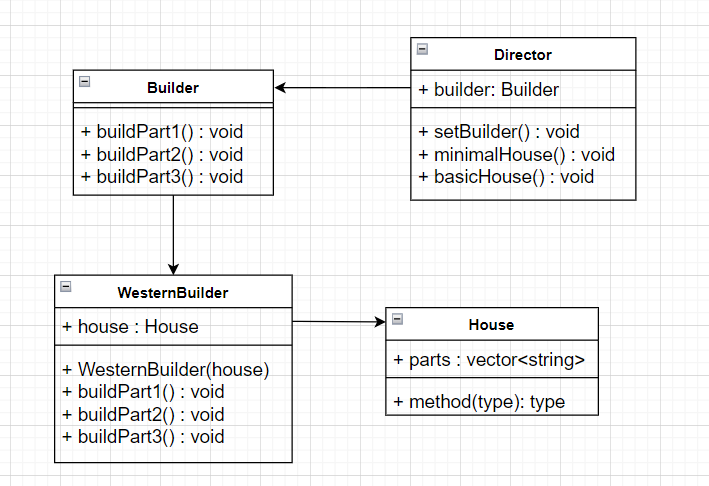
\includegraphics[scale=0.65]{image/creational/bso.png}  
\end{center}
Builder có các thành phần chính sau:
\begin{itemize}
    \item Một abstract class hay interface khai báo trước để định dạng có thể có chung cho các đối tượng sản phẩm. Người ta gọi nó là Builder.
    \item Các class kế thừa từ Builder để cung cấp cách triển khai các bước construction. Các concrete Builder này có thể được dùng để tạo ra các product không tuân theo các khuôn mẫu chung.
    \item Một class Sản phẩm là đối tượng đầu ra của kết quả được tạo nên từ Builder.
    \item Một class Director để xác địng thứ tự gọi các bước contruction.
\end{itemize}
\subsubsection{Ưu điểm và Nhược điểm }
Có thể dễ dàng thấy các ưu nhược điểm như sau:
Ưu điểm:
\begin{itemize}
    \item Builder pattern cho phép bạn xây dựng Object theo nhiều cách khác nhau bằng cách kết hợp các bước xây dựng khác nhau.
    \item Builder pattern tách biệt quy trình xây dựng Object khỏi Object cuối cùng, giúp giảm sự phức tạp của mã và tăng tính Module hóa.
\end{itemize}
Nhược điểm:
\begin{itemize}
    \item Builder pattern có thể tạo ra một lớp Builder và các bước xây dựng riêng biệt, làm tăng độ phức tạp và số lượng mã cần viết. Nếu đối tượng không phức tạp và không có nhiều tham số khác nhau, việc sử dụng Builder pattern có thể làm mã phức tạp.
\end{itemize}
\subsubsection{Code}
\begin{itemize}
    \item Ta có một căn nhà có thể được xây dựng.
    \item Đồng thời là một đội ngũ làm việc để xây dựng nên căn nhà đó. Đặc biệt là đội ngũ xây dựng nhà theo phong cách phương Tây xây nhà chia theo từng khu vực 1,2,3.
    \item Tiếp đó là một Nhà thầu chỉ định xây dựng căn nhà như thế nào.
    \item Có 2 loại nhà là loại nhà đơn giản gồm khu 1 và loại nhà căn bản gồm cả 3 khu nhà.
\end{itemize}
\begin{lstlisting}
#include <iostream>
#include <vector>
using namespace std;

class House
{
public:
    vector<string> parts;
    void show() const
    {
        cout << "House parts: ";
        for (int i = 0; i < parts.size(); i++)
            if (parts[i] == parts.back())
                cout << parts[i];
            else
                cout << parts[i] << ", ";
        cout << "\n\n";
    }
};

class Builder
{
public:
    virtual void buildPart1() = 0;
    virtual void buildPart2() = 0;
    virtual void buildPart3() = 0;
};

class WesternBuilder : public Builder
{
private:
    House *house;

public:
    WesternBuilder() { this->house = new House(); }
    void buildPart1() override { this->house->parts.push_back("Western Part1"); }
    void buildPart2() override { this->house->parts.push_back("Western Part2"); }
    void buildPart3() override { this->house->parts.push_back("Western Part3"); }

public:
    House *getResult() { return this->house; }
};

class Director
{
private:
    Builder *builder;

public:
    void setBuilder(Builder *builder) { this->builder = builder; }
    void minimalHouse() { this->builder->buildPart1(); }
    void basicHouse()
    {
        this->builder->buildPart1();
        this->builder->buildPart2();
        this->builder->buildPart3();
    }
};

int main()
{
    Director *director = new Director();
    WesternBuilder *wbuilder = new WesternBuilder();
    WesternBuilder *wbuilder1 = new WesternBuilder();
    director->setBuilder(wbuilder);
    director->minimalHouse();
    House *house = wbuilder->getResult();
    cout << "--------------minimal House 1-------------" << endl;
    house->show();
    director->setBuilder(wbuilder1);
    director->basicHouse();
    house = wbuilder1->getResult();
    cout << "--------------basic House 2-------------" << endl;
    house->show();
    return 0;
}
\end{lstlisting}
Ở hàm main, ta gọi nhà thầu, và 2 nhà xây dựng phong cách phương Tây khác nhau. Đầu tiên, nhà thầu chỉ định nhà xây dựng một xây nhà và cho ra kết quả, tiếp đó là nhà xây dựng 2 cũng tương tự.\\
\newline
\textbf{Kết quả:}
\begin{lstlisting}
--------------minimal House 1-------------
House parts: Western Part1

--------------basic House 2-------------
House parts: Western Part1, Western Part2, Western Part3    
\end{lstlisting}
\subsubsection{Các Pattern liên quan}
\begin{itemize}
    \item Có thể kết hợp với Composite do Composite cung cấp một hệ thống phân lớp phù hợp với hệ thống xây dựng nên từ các bộ phận nhỏ bằng cấp.
    \item có thể kết hợp với Iterator vì nó cung cấp khả năng duyệt qua các phần từ. Trong trường hợp này là các bước construction.
    \item Visitor cũng là một mẫu có thể được kết hợp vì nó cung cấp cách để thực hiện một hành động mới mà không ảnh hưởng đến mã nguồn của đối tượng. Trong trường hợp này có thể là có một bộ phận nhà có cách xây dựng khác với bình thường.
\end{itemize}
\subsection{Prototype}
\subsubsection{Định nghĩa}
Prototype là một loại Creational Design Pattern cho phép ta sao chép một object đã tồn tại mà không cần đoạn code ở trong chính class đối tượng đó.
\subsubsection{Cách sử dụng}
Thông thường, các trường hợp có thể sử dụng Prototype như sau:
\begin{itemize}
    \item Khi việc tạo một Object mới là một quá trình tốn kém về tài nguyên hoặc thời gian.
    \item Khi bạn muốn tránh việc chỉnh sửa mã nguồn của đối tượng gốc khi tạo ra các bản sao.
\end{itemize}
\subsubsection{Cấu trúc}
Ta có thể giải quyết vấn đề trên như sau:
\begin{itemize}
    \item 1. Tạo ra một interface hoặc abstract class có hàm clone().
    \item 2. Tạo ra một vài subclasses (Concrete Class) con kế thừa từ interface trên và implement lại hàm clone().
    \item 3. Tạo ra đối tượng bằng hàm clone().
    \item 4. Nếu cần thiết ta kết hợp cả phương pháp Factory Method, sử dụng Factory để tạo ra các đối tượng cloned một cách dễ dàng.
\end{itemize}
\begin{center}
    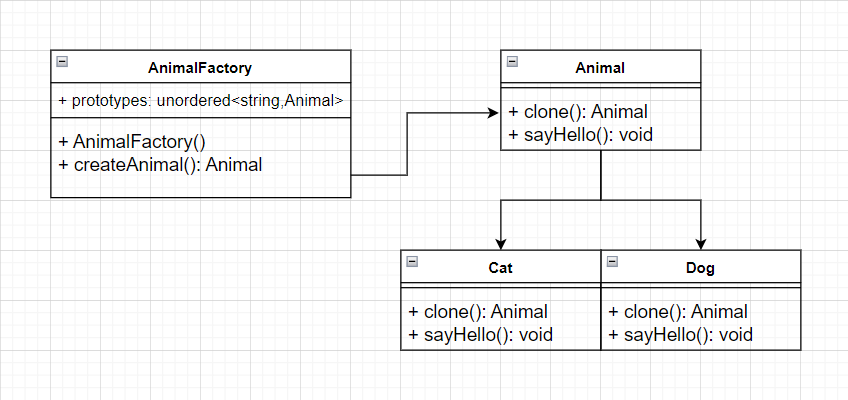
\includegraphics[scale=0.9]{image/creational/pso.png}
\end{center}
Các thành phần chính:
\begin{itemize}
    \item Một interface hay abstract class của đối tượng muốn được khởi tạo chứa hàm clone().
    \item Các Subclass kế thừa từ interface trên và có hàm clone thật chất là sử dụng copy constructor để tạo ra đối tượng mới có giá trị giống hệt đối tượng cũ.
\end{itemize}
\subsubsection{Ưu điểm và Nhược }
Ta thường thấy các ưu nhược điểm sau:\\\\
Ưu điểm:
\begin{itemize}
    \item Prototype pattern cho phép bạn tạo ra các bản sao của Object mà không cần biết lớp cụ thể của đối tượng đó. Điều này giúp giảm thiểu sự phụ thuộc và làm cho hệ thống linh hoạt hơn.
    \item Thay vì tạo ra một Object mới từ đầu, Prototype pattern cho phép sao chép các Object hiện có, giúp tiết kiệm thời gian và tài nguyên. Điều này đặc biệt hữu ích trong việc tạo ra các đối tượng phức tạp hoặc tốn kém về tài nguyên.
\end{itemize}
Nhược điểm:
\begin{itemize}
    \item  Nếu Object có các Object con hoặc liên kết với các tài nguyên khác, việc sao chép Object có thể trở nên khó khăn và mất thời gian.
    \item Đôi khi, các Object không thể hoặc không nên được sao chép. Trong trường hợp này, việc triển khai Prototype pattern có thể gặp khó khăn và không phù hợp.
\end{itemize}
\subsubsection{Code}
\begin{itemize}
    \item Ta có 2 loại động vật là chó và mèo.
    \item Một nhà máy để tạo ra một đối tượng được sao chép từ đối tượng đã được khởi tạo.
\end{itemize}
\begin{lstlisting}
#include <iostream>
#include <string>
#include <unordered_map>

using namespace std;

// Base class for prototype objects
class Animal
{
public:
    virtual Animal *clone() = 0;
    virtual void sayHello() = 0;
};

// Concrete prototype classes
class Dog : public Animal
{
public:
    Animal *clone() override { return new Dog(*this); }
    void sayHello() override { cout << "Woof!" << endl; }
};

class Cat : public Animal
{
public:
    Animal *clone() override { return new Cat(*this); }
    void sayHello() override { cout << "Meow!" << endl; }
};

// Prototype factory class
class AnimalFactory
{
public:
    AnimalFactory()
    {
        prototypes["dog"] = new Dog();
        prototypes["cat"] = new Cat();
    }

    Animal *createAnimal(string type) { return prototypes[type]->clone(); }

private:
    unordered_map<string, Animal *> prototypes;
};

int main()
{
    AnimalFactory factory;

    Animal *dog1 = factory.createAnimal("dog");
    Animal *dog2 = factory.createAnimal("dog");
    Animal *cat1 = factory.createAnimal("cat");
    Animal *cat2 = factory.createAnimal("cat");

    dog1->sayHello(); // outputs "Woof!"
    dog2->sayHello(); // outputs "Woof!"
    cat1->sayHello(); // outputs "Meow!"
    cat2->sayHello(); // outputs "Meow!"

    return 0;
} 
\end{lstlisting}
Ở hàm main, ta tạo ra đối tượng chó rồi tạo ra đối tượng được copy chó, và tương tự với đối tượng mèo.\\
\newline
\textbf{Kết quả:}
\begin{lstlisting}
Woof!
Woof!
Meow!
Meow!
\end{lstlisting}
\subsubsection{Các Pattern liên quan}
\begin{itemize}
    \item Factory và Abstract Factory ít nhiều có thể cần tạo ra các clone của nó.
    \item Commands có thể được sao lưu ở nhiều nơi.
    \item Decorator cũng có thể sử dụng để sao chép ra đối tượng mới rồi áp dụng decorator lên nó.
\end{itemize}
\subsection{Singleton}
\subsubsection{Định nghĩa}
Singleton là một Creational Pattern cho phép chúng ta chỉ có duy nhất một đối tượng được khởi tạo và sử dụng xuyên suốt chương trình của một class.
\subsubsection{Cách sử dụng}
Thông thường, các trường hợp có thể sử dụng Singleton như sau:
\begin{itemize}
    \item Khi bạn chỉ muốn có một đối tượng duy nhất của một lớp và muốn truy cập đến nó từ mọi nơi trong ứng dụng.
    \item Khi việc tạo lại đối tượng từ đầu mất thời gian và tài nguyên, và bạn muốn tái sử dụng đối tượng đã có.
\end{itemize}
\subsubsection{Cấu trúc}
Để có thể dễ dàng thực thi Singleton Pattern, ta thực hiện theo các bước sau:
\begin{itemize}
    \item 1. Để constructor private để ngăn các objects khác sử dụng từ khóa \textbf{new} với class Singleton.
    \item 2. Tạo một phương thức khởi tạo static mới để thay thế vai trò của constructor. Phương thức này gọi hàm constructor private để khởi tạo đối tượng và lưu đối tượng đó dưới dạng static. Tất cả các lần gọi tiếp theo đều trả về đối tượng đã được tạo static này.
\end{itemize}
\begin{center}
    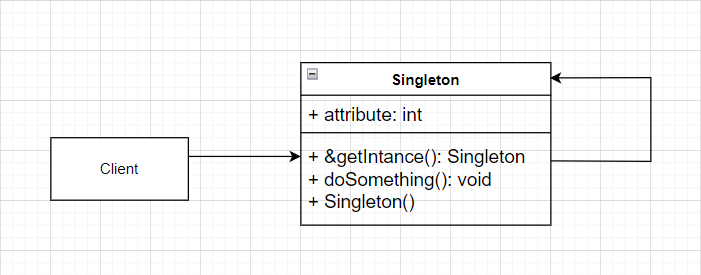
\includegraphics[]{image/creational/sso.png}
\end{center}
Các thành phần chính:
\begin{itemize}
    \item Các class khởi tạo đối tượng duy nhất chỉ định hàm constructor về private.
\end{itemize}
\subsubsection{Ưu điểm và Nhược điểmđiểm}
Ta thường thấy các ưu nhược điểm sau:\\\\
Ưu điểm:
\begin{itemize}
    \item Singleton đảm bảo rằng chỉ có một đối tượng duy nhất của lớp tồn tại trong suốt vòng đời của ứng dụng. Điều này đảm bảo rằng mọi truy cập đến đối tượng này đều nhận được cùng một thể hiện.
    \item Vì Singleton có phạm vi toàn cục trong ứng dụng, bạn có thể truy cập đến nó từ mọi nơi trong mã của bạn. Điều này giúp bạn dễ dàng chia sẻ thông tin và trạng thái giữa các phần khác nhau của ứng dụng.
    \item Singleton giúp bạn tiết kiệm tài nguyên bằng cách tái sử dụng một đối tượng đã có thay vì tạo ra một đối tượng mới mỗi khi cần sử dụng.
\end{itemize}
Nhược điểm:
\begin{itemize}
    \item Do Singleton tồn tại trong suốt vòng đời của ứng dụng, việc kiểm tra và kiểm soát đối tượng Singleton có thể trở nên khó khăn..
    \item Singleton có thể gây ra xung đột trong môi trường đa luồng hoặc trong trường hợp nhiều luồng cố gắng truy cập và sửa đổi đối tượng Singleton cùng một lúc. Cần phải chú ý đến việc đồng bộ hóa để tránh xung đột.
\end{itemize}
\subsubsection{Code}
\begin{itemize}
    \item Ta có một đối tượng duy nhất chỉ được khởi tạo một lần (class Singleton), lưu ý, ta để constructor ở trạng thái private.
    \item Ở class Singleton, ta có một phương thức static là getInstance() để kêu đối tượng được khởi tạo ban đầu ở mọi nơi trong code của chúng ta.
\end{itemize}
\begin{lstlisting}
#include <iostream>

using namespace std;

class Singleton
{
public:
    int attribute = 0;

public:
    static Singleton &getInstance()
    {

        static Singleton instance; // static local variable
        return instance;
    }

    void doSomething()
    {
        attribute++;
        cout << "attribute: " << attribute << endl;
    }

private:
    Singleton()
    {
        // private constructor to prevent direct instantiation
        cout << "Creating Singleton instance..." << endl;
    }

    ~Singleton()
    {
        // private destructor to prevent deletion of the instance
        cout << "Destroying Singleton instance..." << endl;
    }

    // private copy constructor and assignment operator to prevent cloning
    Singleton(const Singleton &) = delete;
    Singleton &operator=(const Singleton &) = delete;
};

int main()
{
    Singleton &singleton = Singleton::getInstance();
    singleton.doSomething();
    Singleton &singleton2 = Singleton::getInstance();
    singleton2.doSomething();

    return 0;
}

\end{lstlisting}
Ở hàm main, ta đầu tiên tạo ra đối tượng singleton, và thực hiện việc cộng biến lên 1 đơn vị. Sau đó, ta tiếp tục khởi tạo đối tượng mới tuy nhiên vẫn là gọi lại đối tượng cũ, và sau đó là thực hiện hành vi cộng biến lên 1 đơn vị và kết quả cho ra sẽ là 2.\\
\newline
\textbf{Kết quả:}
\begin{lstlisting}
Creating Singleton instance...
attribute: 1
attribute: 2
Destroying Singleton instance...
\end{lstlisting}
\newpage
\section{Structural Patterns}
Ở phần Structural Patterns, ta có 7 mẫu Patterns cụ thể là \textbf{Adapter}, \textbf{Bridge}, \textbf{Composite}, \textbf{Decorator}, \textbf{Facade}, \textbf{Flyweight}, \textbf{Proxy}. Nhờ vào 7 mẫu này mà ta có thể thiết lập quan hệ giữa các đối tượng với nhau.\\
\subsection{Adapter}
\subsubsection{Định nghĩa}
Adapter là một Structural Pattern cung cấp cho bạn thiết kế có thể phối hợp hai đối tượng với lớp cha kế thừa interface không tương thích nhau.
\subsubsection{Cách sử dụng}
Bạn nên sử dụng Adapter trong các trường hợp sau:
\begin{itemize}
    \item Khi bạn muốn kết nối hai lớp hoặc hệ thống không tương thích với nhau về giao diện.
    \item Khi bạn muốn tái sử dụng lại một lớp đã tồn tại trong một hệ thống mới mà không cần chỉnh sửa lớp đó.
\end{itemize}
\subsubsection{Cấu trúc}
\begin{itemize}
    \item ImageViewer có vai trò như adapter để chuyển đổi sang các dạng cần thiết để hiển thị.
\end{itemize}
\begin{center}
    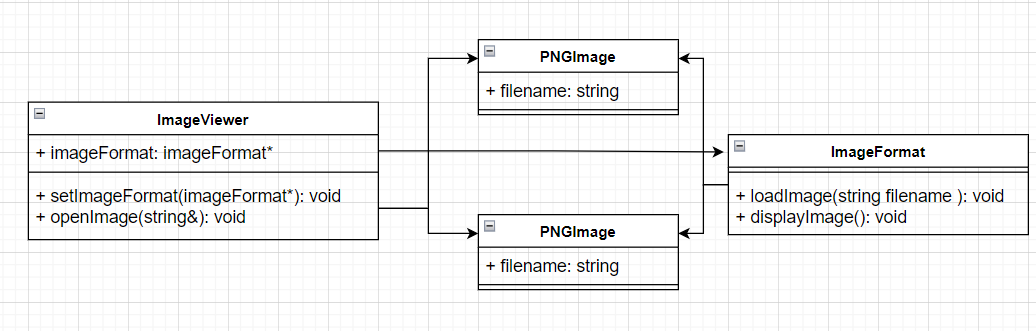
\includegraphics[scale=0.75]{image/structural/adapter.png}
\end{center}
Các thành phần chính:
\begin{itemize}
    \item Một class mô tả một giao thức mà các lớp khải phải tuân theo để hoạt động.
    \item Một Adapter để chuyển đối cách hoạt động của các hàm.
    \item Một class Service để thực hiện các hành vi cần thiết.
\end{itemize}
\subsubsection{Ưu điểm và Nhược điểm}
Ta có các ưu và nhược điểm dễ thấy sau:\\\\
Ưu điểm:
\begin{itemize}
    \item Adapter giúp kết nối các lớp hoặc hệ thống không tương thích với nhau về giao diện và cho phép chúng làm việc cùng nhau.
    \item Adapter cho phép tái sử dụng lại các lớp đã tồn tại và mở rộng chức năng của chúng mà không cần thay đổi lớp gốc.
\end{itemize}
Nhược điểm:
\begin{itemize}
    \item Adapter không thể giải quyết các trường hợp tương thích mạnh hơn, trong đó sự khác biệt giữa các giao diện là quá lớn để có thể chuyển đổi trực tiếp.
\end{itemize}
\subsubsection{Code Example}
\begin{itemize}
    \item Ta có 2 loại hình ảnh là Png và Jpeg.
    \item Các loại hình ảnh có 2 phương thức là tải hình ảnh lên và hiển thị hình ảnh.
    \item Ta có giao diện người xem sẽ chứa thuộc tính format của loại hình ảnh hoạt động như một adapter để chuyển qua lại loại hình ảnh nhờ hàm setImageFormat().
\end{itemize}
\begin{lstlisting}
#include <iostream>
#include <string>

class ImageFormat {
public:
    virtual void loadImage(const std::string& filename) = 0;
    virtual void displayImage() = 0;
};

class PNGImage : public ImageFormat {
private:
    std::string filename;

public:
    void loadImage(const std::string& filename) override {
        this->filename = filename;
        std::cout << "Loading PNG image: " << filename << std::endl;
    }

    void displayImage() override {
        std::cout << "Displaying PNG image: " << filename << std::endl;
    }
};

class JPEGImage : public ImageFormat {
private:
    std::string filename;

public:
    void loadImage(const std::string& filename) override {
        this->filename = filename;
        std::cout << "Loading JPEG image: " << filename << std::endl;
    }

    void displayImage() override {
        std::cout << "Displaying JPEG image: " << filename << std::endl;
    }
};

class ImageViewer {
private:
    ImageFormat* imageFormat;

public:
    void setImageFormat(ImageFormat* format) {
        imageFormat = format;
    }

    void openImage(const std::string& filename) {
        imageFormat->loadImage(filename);
        imageFormat->displayImage();
    }
};

int main() {
    ImageViewer viewer;

    viewer.setImageFormat(new PNGImage());
    viewer.openImage("image.png");

    viewer.setImageFormat(new JPEGImage());
    viewer.openImage("image.jpg");

    return 0;
}

\end{lstlisting}
Ở hàm main, ta gọi một giao diện người dùng và lần lượt chỉnh giao diện đó thành loại hình ảnh Png và Jpeg và mở lần lượt xen kẻ.\\
\newline
\textbf{Kết quả:}
\begin{lstlisting}
Loading PNG image: image.png
Displaying PNG image: image.png
Loading JPEG image: image.jpg
Displaying JPEG image: image.jpg
\end{lstlisting}
\subsubsection{Các Pattern liên quan}
\begin{itemize}
    \item Bride: có cấu trúc khá giống với Adapter nhưng khác nhau về mặt sử dụng.
    \item Decorator: hoặc ta có thể tăng cường class cần chuyển đối bằng decorator.
    \item Proxy: hoặc có thể tạo một Proxy class tương ứng với sản phẩm để nó tương tác với người dùng và chuyển đối qua Proxy khác trước khi truy cập trực tiếp vào đối tượng chính.
\end{itemize}
\subsection{Bridge}
\subsubsection{Định nghĩa}
Bridge pattern là một mẫu thiết kế thuộc nhóm cấu trúc (structural pattern) trong lập trình hướng đối tượng. Nó giúp tách biệt abstraction (abstraction) và implementation (implementation), cho phép chúng được phát triển độc lập và có thể thay đổi mà không ảnh hưởng đến nhau.
\subsubsection{Cách sử dụng}
Sử dụng Bridge Patern khi chúng ta muốn:
\begin{itemize}
    \item Khi bạn muốn tách rời abstraction và implementation để chúng có thể thay đổi một cách độc lập.
    \item Khi bạn muốn có khả năng mở rộng và thêm các implementation mới mà không ảnh hưởng đến abstraction hiện có.
\end{itemize}
\subsubsection{Cấu trúc}
Các thành phần chính:
\begin{itemize}
    \item Một interface hay abstract class định nghĩa các đối tượng liên quan.
    \item Một loạt các subclass kế thừa từ interface để tạo ra các loại sản phẩm.
    \item Một interface định nghĩa một cách hoạt động chung.
    \item Một loạt các class kế thừa từ interface để cụ thể hóa việc thực thi.
\end{itemize}
\begin{center}
    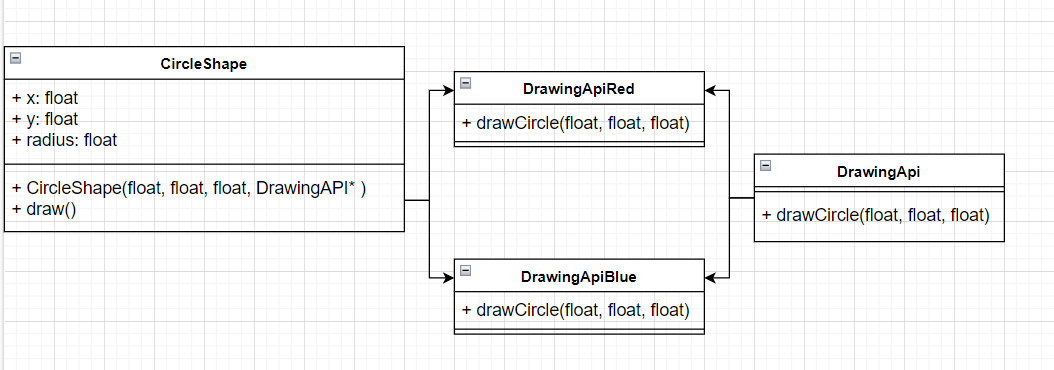
\includegraphics[scale=0.7]{image/structural/bridge.png}
\end{center}
\begin{itemize}
    \item Ở đây, CirceShape là một Concrete Class của Shape thuộc Abtraction Class, có thêm nhiều class như thế này vào không thành vấn đề.
    \item DrawingApi là một Implementation Class các Subclass của class này sẽ cụ thể thực hiện hành động như thế nào với các subclass của abstraction class. Bạn có thể thêm thoải mái các class như thế này.
\end{itemize}
\subsubsection{Ưu điểm và Nhược điểm}
Ta có các ưu và nhược điểm dễ thấy sau:\\\\
Ưu điểm:
\begin{itemize}
    \item Tách biệt abstraction và implementation, giúp giảm sự phức tạp và khả năng linh hoạt hơn trong việc thay đổi và mở rộng các thành phần.
    \item Các lớp abstraction và implementation có thể được mở rộng một cách độc lập, cho phép thêm mới các subclass mà không ảnh hưởng đến nhau.
\end{itemize}
Nhược điểm:
\begin{itemize}
    \item Đôi khi việc tách rời abstraction và implementation có thể tạo ra sự phức tạp thêm cho hệ thống nếu không được sử dụng một cách hợp lý.
\end{itemize}
\subsubsection{Code Example}
\begin{itemize}
    \item Có một loại hình duy nhấ là hình tròn.
    \item Có 2 cách vẽ với 2 màu khác nhau.
\end{itemize}
\begin{lstlisting}
#include <iostream>

// Abstraction
class Shape {
protected:
    class DrawingAPI* drawingAPI;

public:
    Shape(DrawingAPI* api) : drawingAPI(api) {}
    virtual void draw() = 0;
};

// Implementation
class DrawingAPI {
public:
    virtual void drawCircle(float x, float y, float radius) = 0;
};

// Concrete Implementation 1
class DrawingAPIRed : public DrawingAPI {
public:
    void drawCircle(float x, float y, float radius) {
        std::cout << "Red circle at (" << x << "," << y << ") radius " << radius << std::endl;
    }
};

// Concrete Implementation 2
class DrawingAPIBlue : public DrawingAPI {
public:
    void drawCircle(float x, float y, float radius) {
        std::cout << "Blue circle at (" << x << "," << y << ") radius " << radius << std::endl;
    }
};

// Refined Abstraction
class CircleShape : public Shape {
private:
    float x, y, radius;

public:
    CircleShape(float x, float y, float radius, DrawingAPI* api) : Shape(api), x(x), y(y), radius(radius) {}

    void draw() {
        drawingAPI->drawCircle(x, y, radius);
    }
};

int main() {
    DrawingAPIRed drawingAPIred;
    DrawingAPIBlue drawingAPIblue;

    CircleShape circle1(1, 2, 3, &drawingAPIred);
    CircleShape circle2(4, 5, 6, &drawingAPIblue);

    circle1.draw();
    circle2.draw();

    return 0;
}

\end{lstlisting}
Ở hàm main, ta thực hiện gọi 2 api để vẽ hình tròn với 2 màu khác nhau.\\
\newline
\textbf{Kết quả:}
\begin{lstlisting}
Red circle at (1,2) radius 3
Blue circle at (4,5) radius 6
\end{lstlisting}
\subsubsection{Các Pattern liên quan}
\begin{itemize}
    \item Adapter và Bride giống nhau về cấu trúc nhưng khác nhau về mục đích sử dụng.
    \item Abstract Factory: việc ghép nối này là hữu ích vì các Abstraction trong Bridge trong một số trường hợp chỉ có thể hoạt động được với các triển khai cụ thể nên việc đóng gói của Abstract Factory là cần thiết.
    \item Builder: Director giữ vai trò của Abstraction và các Builder giũ vai trò của Implementation.
\end{itemize}
\subsection{Composite}
\subsubsection{Định nghĩa}
Composite là một mẫu thiết kế thuộc nhóm cấu trúc (structural design pattern) trong lập trình hướng đối tượng. Mẫu thiết kế này cho phép bạn tạo ra cấu trúc cây đặc biệt, gồm các đối tượng con và đối tượng tổng hợp chung một giao diện chung. Composite cho phép các đối tượng con và đối tượng tổng hợp được xử lý một cách đồng nhất, không phân biệt.
\subsubsection{Cách sử dụng}
Hãy sử dụng khi:
\begin{itemize}
    \item Khi bạn muốn thực hiện các hoạt động chung cho tất cả các đối tượng trong cây mà không cần kiểm tra kiểu của chúng.
    \item Khi bạn muốn tạo ra các đối tượng trong các cấu trúc cây để biểu diễn hệ thống phân lớp.
\end{itemize}
\subsubsection{Cấu trúc}
\begin{center}
    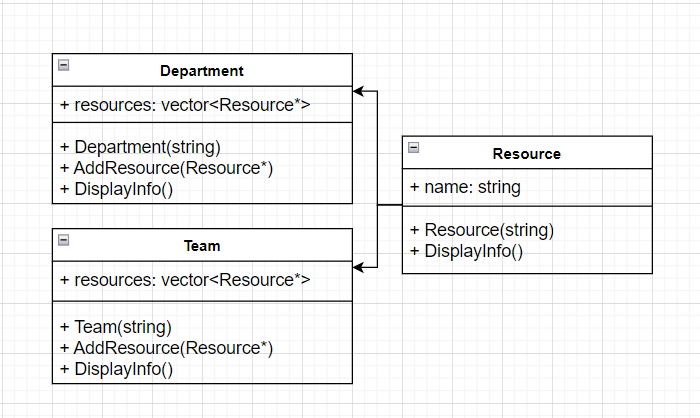
\includegraphics[scale=0.7]{image/structural/composite.png}
\end{center}
Các thành phần chính bao gồm:
\begin{itemize}
    \item Component: là một interface hoặc abstract class định nghĩa chung cho các thành phần con tham gia trong cây.
    \item Leaf: là các lớp thực hiện các phương thức của component, không có subclass.
    \item Composite: lưu trữ các Leaf và các phương thức của Component đồng thời ủy nhiệm nhiệm vụ thực hiện cho các Leaf.
\end{itemize}
\subsubsection{Ưu điểm và Nhược điểm}
Ta có các ưu và nhược điểm dễ thấy sau:\\\\
Ưu điểm:
\begin{itemize}
    \item Composite cho phép bạn xử lý các đối tượng con và đối tượng tổng hợp theo cách thống nhất, mà không phải phân biệt giữa chúng.
    \item Bạn có thể dễ dàng thêm mới các đối tượng con vào cây mà không ảnh hưởng đến cấu trúc tổng thể của cây.
\end{itemize}
Nhược điểm:
\begin{itemize}
    \item Có thể gây ra hiệu năng giảm đối với các cây rất lớn do việc duyệt qua toàn bộ cấu trúc.
\end{itemize}
\subsubsection{Code Example}
\begin{itemize}
    \item Một công ty có các rất nhiều bộ phận liên kết với nhau tạo thành một cây hoàn chỉnh.
\end{itemize}
\begin{lstlisting}
#include <iostream>
#include <string>
#include <vector>

namespace Company {
    class Resource {
    protected:
        std::string name;

    public:
        Resource(const std::string& name) : name(name) {}

        virtual void DisplayInfo() const = 0;
    };

    class Department : public Resource {
    private:
        std::vector<Resource*> resources;

    public:
        Department(const std::string& name) : Resource(name) {}

        void AddResource(Resource* resource) {
            resources.push_back(resource);
        }

        void DisplayInfo() const override {
            std::cout << "Department: " << name << std::endl;
            for (const auto& resource : resources) {
                resource->DisplayInfo();
            }
        }
    };

    class Team : public Resource {
    private:
        std::vector<Resource*> resources;

    public:
        Team(const std::string& name) : Resource(name) {}

        void AddResource(Resource* resource) {
            resources.push_back(resource);
        }

        void DisplayInfo() const override {
            std::cout << "Team: " << name << std::endl;
            for (const auto& resource : resources) {
                resource->DisplayInfo();
            }
        }
    };

    class Employee : public Resource {
    private:
        std::string position;

    public:
        Employee(const std::string& name, const std::string& position) : Resource(name), position(position) {}

        void DisplayInfo() const override {
            std::cout << "Employee: " << name << " (Position: " << position << ")" << std::endl;
        }
    };

    class Project : public Resource {
    private:
        std::string status;

    public:
        Project(const std::string& name, const std::string& status) : Resource(name), status(status) {}

        void DisplayInfo() const override {
            std::cout << "Project: " << name << " (Status: " << status << ")" << std::endl;
        }
    };
}

int main() {
    using namespace Company;

    Department* developmentDepartment = new Department("Development Department");

    Team* team1 = new Team("Team 1");
    Employee* employee1 = new Employee("John Doe", "Software Engineer");
    Employee* employee2 = new Employee("Jane Smith", "UI/UX Designer");
    team1->AddResource(employee1);
    team1->AddResource(employee2);

    Team* team2 = new Team("Team 2");
    Employee* employee3 = new Employee("Mike Johnson", "Backend Developer");
    Employee* employee4 = new Employee("Emily Davis", "Frontend Developer");
    team2->AddResource(employee3);
    team2->AddResource(employee4);

    developmentDepartment->AddResource(team1);
    developmentDepartment->AddResource(team2);

    Project* project1 = new Project("Project A", "In Progress");
    Project* project2 = new Project("Project B", "Completed");

    developmentDepartment->AddResource(project1);
    developmentDepartment->AddResource(project2);

    developmentDepartment->DisplayInfo();

    delete developmentDepartment;
    delete team1;
    delete team2;
    delete employee1;
    delete employee2;
    delete employee3;
    delete employee4;
    delete project1;
    delete project2;

    return 0;
}

\end{lstlisting}
Ở hàm main, ta tạo team1 và thêm 2 nhân viên vào đó. Ta tạo team 2 và thêm 2 nhân viên vào đó. Bộ phận phát triển thêm 2 team này vào nó. Bộ phận phát triển cũng thêm vào 2 dư án vừa được tạo. Sau cùng hiển thị ra toàn bộ.\\
\newline
\textbf{Kết quả:}
\begin{lstlisting}
Department: Development Department
Team: Team 1
Employee: John Doe (Position: Software Engineer)
Employee: Jane Smith (Position: UI/UX Designer)
Team: Team 2
Employee: Mike Johnson (Position: Backend Developer)
Employee: Emily Davis (Position: Frontend Developer)
Project: Project A (Status: In Progress)
Project: Project B (Status: Completed)

\end{lstlisting}
\subsubsection{Các Pattern liên quan}
\begin{itemize}
    \item Builder: kết hợp với builder để tạo ra cây phức tạp nhiều tầng.
    \item Chain of Responsibility: thường phối hợp chung với Composite có thể dễ dàng thấy vì tính tương đồng ở cấu trúc.
    \item Dùng Iterator để duyệt con.
    \item Dùng Visitor để thực hiện hành động đặc biệt trên toàn bộ cây.
    \item Flyweight: tiết kiệm dung lượng ram do việc tạo ra cây khá tốn bộ nhớ.
    \item Dùng Decorator để trang trí các thành phần con nếu cần.
    \item Dùng Prototype để clone() con hoặc clone() cả cây.
\end{itemize}
\subsection{Decorator}
\subsubsection{Định nghĩa}
Decorator là một mẫu thiết kế cấu trúc (structural design pattern) cho phép bổ sung các tính năng mới vào một đối tượng mà không làm thay đổi cấu trúc của lớp gốc. Nó cho phép mở rộng chức năng của một đối tượng bằng cách đóng gói nó vào trong một lớp decorator mới và gắn kết chúng với nhau theo cấu trúc lồng nhau.
\subsubsection{Cách sử dụng}
Chúng ta sẽ sử dụng Decorator khi:
\begin{itemize}
    \item Khi muốn thêm tính năng mới cho các đối tượng mà không ảnh hưởng đến các đối tượng này.
    \item Khi bạn muốn mở rộng chức năng của một đối tượng mà không ảnh hưởng đến các đối tượng khác cùng loại.
    \item Khi không thể mở rộng một đối tượng bằng cách thừa kế (inheritance). Chẳng hạn, một class sử dụng từ khóa final, muốn mở rộng class này chỉ còn cách duy nhất là sử dụng decorator.
\end{itemize}
\subsubsection{Cấu trúc}
Các thành phần chính:
\begin{itemize}
    \item Một interface quy định mẫu dùng chung cho các sản phẩm
    \item Các sản phẩm kế thừa interface.
    \item Một abstract class có tham chiếu đến đối tượng sản phẩm và phương thức của interface quy định mẫu sản phẩm.
    \item Các Decorator con được kế thừa.
\end{itemize}
\begin{center}
    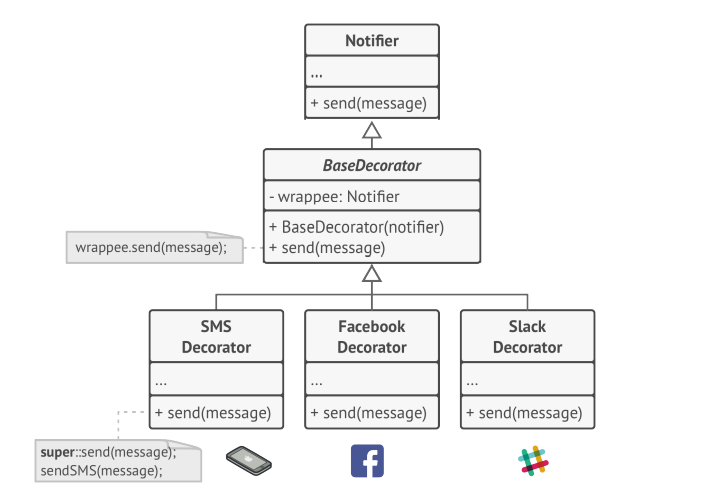
\includegraphics[scale=0.6]{image/structural/decorator.png}
\end{center}
\begin{itemize}
    \item Kiển trúc này thực chất là sau mỗi lần kế thừa, ta thêm vào các thuộc tính hoặc làm mới hàm mà vẫn giữ các giá trị của hảm cũ thì đó gọi là decorator.
\end{itemize}
\subsubsection{Ưu điểm và Nhược điểm}
Ta có các ưu và nhược điểm dễ thấy sau:\\\\
Ưu điểm:
\begin{itemize}
    \item Cho phép mở rộng chức năng của một đối tượng mà không làm thay đổi cấu trúc của lớp gốc.
    \item Có thể kết hợp nhiều decorator để tạo ra các kết hợp chức năng phức tạp.
    \item Bạn có thể mở rộng hành vi của đối tượng mà không cần tạo lớp con mới.
    \item Cung cấp tính linh hoạt và tùy chỉnh cao khi thêm hoặc xóa chức năng mà không ảnh hưởng đến các đối tượng khác.
\end{itemize}
Nhược điểm:
\begin{itemize}
    \item Dễ dẫn đến việc tạo ra quá nhiều lớp decorator nhỏ, dẫn đến sự phức tạp và khó khăn trong việc quản lý.
\end{itemize}
\subsubsection{Code Example}
\begin{itemize}
    \item Có 1 loại nước uống là Coffee.
    \item Có 2 loại trang trí đi kèm là Milk và Sugar.
\end{itemize}
\begin{lstlisting}
#include <iostream>
#include <string>

// Component interface
class Beverage {
public:
    virtual std::string getDescription() const = 0;
    virtual double getCost() const = 0;
};

// Concrete component
class Coffee : public Beverage {
public:
    std::string getDescription() const override {
        return "Coffee";
    }

    double getCost() const override {
        return 2.0;
    }
};

// Decorator
class BeverageDecorator : public Beverage {
protected:
    Beverage* beverage;

public:
    BeverageDecorator(Beverage* beverage) : beverage(beverage) {}

    std::string getDescription() const override {
        return beverage->getDescription();
    }

    double getCost() const override {
        return beverage->getCost();
    }
};

// Concrete decorators
class MilkDecorator : public BeverageDecorator {
public:
    MilkDecorator(Beverage* beverage) : BeverageDecorator(beverage) {}

    std::string getDescription() const override {
        return beverage->getDescription() + ", Milk";
    }

    double getCost() const override {
        return beverage->getCost() + 0.5;
    }
};

class SugarDecorator : public BeverageDecorator {
public:
    SugarDecorator(Beverage* beverage) : BeverageDecorator(beverage) {}

    std::string getDescription() const override {
        return beverage->getDescription() + ", Sugar";
    }

    double getCost() const override {
        return beverage->getCost() + 0.25;
    }
};

int main() {
    Beverage* coffee = new Coffee();
    std::cout << "Order: " << coffee->getDescription() << std::endl;
    std::cout << "Cost: $" << coffee->getCost() << std::endl;

    Beverage* coffeeWithMilk = new MilkDecorator(coffee);
    std::cout << "Order: " << coffeeWithMilk->getDescription() << std::endl;
    std::cout << "Cost: $" << coffeeWithMilk->getCost() << std::endl;

    Beverage* coffeeWithMilkAndSugar = new SugarDecorator(coffeeWithMilk);
    std::cout << "Order: " << coffeeWithMilkAndSugar->getDescription() << std::endl;
    std::cout << "Cost: $" << coffeeWithMilkAndSugar->getCost() << std::endl;

    delete coffee;
    delete coffeeWithMilk;
    delete coffeeWithMilkAndSugar;

    return 0;
}

\end{lstlisting}
Ở hàm main, ta gọi 1 tách cà phê và xem thông tin của nó. Sau đó, tiếp tục gọi 1 tách cà phê thêm đường. Cuối cùng là 1 tách cà phê thêm đường và sửa.\\
\newline
\textbf{Kết quả:}
\begin{lstlisting}
Order: Coffee
Cost: $2
Order: Coffee, Milk
Cost: $2.5
Order: Coffee, Milk, Sugar
Cost: $2.75

\end{lstlisting}
\subsubsection{Các Pattern liên quan}
\begin{itemize}
    \item Adapter: Decorator thực chất không hề thay đối nội dung của đối tượng mà mở rộng hay thay đối trách nhiệm của đối tượng đó.
    \item Composite: khá giống nhau về mặt cấu trúc tuy nhiên decorator thêm các hành vi cụ thể hoặc cải tiến nó còn composite thì không.
    \item Strategy cho phép bạn thay đối nội dung của đối tượng trong khi decorator vẫn giữ nguyên.
\end{itemize}
\subsection{Facade}
\subsubsection{Định nghĩa}
Facade là một mẫu thiết kế (design pattern) thuộc nhóm cấu trúc (structural pattern) trong lập trình hướng đối tượng. Facade Pattern cung cấp cho chúng ta một giao diện chung đơn giản thay cho một nhóm các giao diện có trong một hệ thống con (subsystem). Facade Pattern định nghĩa một giao diện ở cấp độ cao hơn để giúp cho người dùng có thể dễ dàng sử dụng hệ thống con này..
\subsubsection{Cách sử dụng}
Chúng ta sẽ sử dụng Fancade trong trường hợp:
\begin{itemize}
    \item Khi có rất nhiều hệ thống con mà mỗi hệ thống con đó lại có những giao diện riêng lẻ của nó nên rất khó cho việc sử dụng phối hợp.
    \item Khi bạn muốn giảm sự phụ thuộc giữa các thành phần của hệ thống và người sử dụng bên ngoài.
    \item Khi bạn muốn tạo ra một lớp bao bọc (wrapper) để ẩn đi chi tiết bên trong và cung cấp một giao diện đơn giản và rõ ràng.
\end{itemize}
\subsubsection{Cấu trúc}
\begin{itemize}
    \item Thực chất, Facade là gôm tất cả các class cùng loại vào một class để dễ sử dụng.
    \item Có thể có nhiều lớp Facde để phục vụ mục đích giải quyết bài toán.
\end{itemize}
Các thành phần chính:
\begin{itemize}
    \item Một hệ thống các sản phẩm kế thừa phức tạp và các chức năng của nó.
    \item Một Facde class biết được hệ thống nào sẽ đáp ứng yêu cầu nào của người dùng.
    \item Một Additonal Facade được tạo ra để phân lớp giúp Facade đỡ phức tạp.
\end{itemize}
\begin{center}
    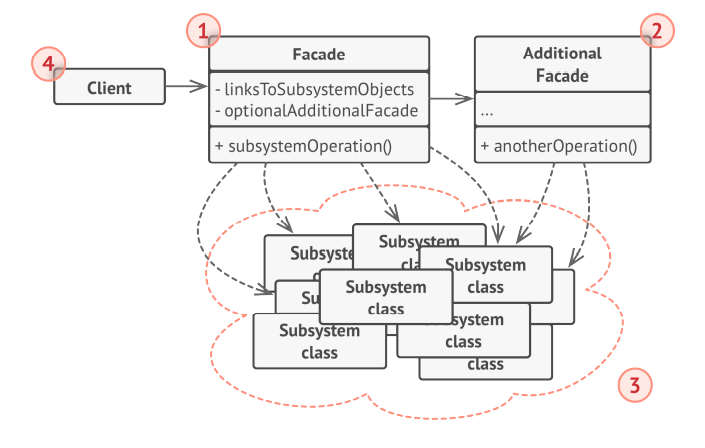
\includegraphics[scale=0.5]{image/structural/facade.png}
\end{center}

\subsubsection{Ưu điểm và Nhược điểm}
Có rất nhiều ưu nhược điểm dễ thấy như sau:\\\\
Ưu điểm:
\begin{itemize}
    \item Ta có thể tách mã nguồn của mình ra khỏi sự phức tạp của hệ thống con.
    \item Có thể đóng gói nhiều hàm được thiết kế không tốt bằng 1 hàm có thiết kế tốt hơn.
    \item Giảm sự phụ thuộc giữa các thành phần của hệ thống, tạo sự tách biệt và khả năng mở rộng cao.
\end{itemize}
Nhược điểm:
\begin{itemize}
    \item Không nên sử dụng quá nhiều lớp Facade với các phương thức phức tạp, vì điều này có thể làm cho giao diện trở nên rườm rà và khó hiểu.
    \item Việc sử dụng Facade cho các hệ thống đơn giản, ko quá phức tạp trở nên dư thừa.
\end{itemize}

\subsubsection{Code Example}
\begin{itemize}
    \item Có 3 loại hình là hình chữ nhật, hình tròn, hình tam giác. Mỗi hình có 2 phương thức là vẽ và xóa.
    \item Có 1 ShapeFacade gom cả 3 hình này vào thành thuộc tính và có 3x2 phương thức là 6 để vẽ và xóa cho mỗi loại hình.
\end{itemize}
\begin{lstlisting}
#include <iostream>

// Rectangle
class Rectangle {
public:
    void draw() {
        std::cout << "Draw rectangle" << std::endl;
    }

    void erase() {
        std::cout << "Erase rectangle" << std::endl;
    }
};

// Circle
class Circle {
public:
    void draw() {
        std::cout << "Draw circle" << std::endl;
    }

    void erase() {
        std::cout << "Erase circle" << std::endl;
    }
};

// Triangle
class Triangle {
public:
    void draw() {
        std::cout << "Draw triangle" << std::endl;
    }

    void erase() {
        std::cout << "Erase triangle" << std::endl;
    }
};

// Facade
class ShapeFacade {
private:
    Rectangle rectangle;
    Circle circle;
    Triangle triangle;

public:
    void drawRectangle() {
        rectangle.draw();
    }

    void eraseRectangle() {
        rectangle.erase();
    }

    void drawCircle() {
        circle.draw();
    }

    void eraseCircle() {
        circle.erase();
    }

    void drawTriangle() {
        triangle.draw();
    }

    void eraseTriangle() {
        triangle.erase();
    }
};

int main() {
    ShapeFacade facade;

    facade.drawRectangle();
    facade.eraseRectangle();

    facade.drawCircle();
    facade.eraseCircle();

    facade.drawTriangle();
    facade.eraseTriangle();

    return 0;
}


\end{lstlisting}
Ở hàm main, ta gọi facade và kêu tất cả các hàm có trong facade.\\
\newline
\textbf{Kết quả:}
\begin{lstlisting}
Draw rectangle
Erase rectangle
Draw circle
Erase circle
Draw triangle
Erase triangle
\end{lstlisting}
\subsubsection{Các Pattern liên quan}
\begin{itemize}
    \item Facade khi kết hợp với Abstract Factory có thể ẩn đi hệ thống được sử dụng để gọi ra sản phẩm.
    \item Adapter và Facade khác nhau ở chỗ Adapter sử dụng mã nguồn này thay vì mã nguồn kia còn Facade gôm hết tất cả lại.
    \item Các đối tượng Facade có thể là Singleton vì nó bao gồm toàn bộ các Subsystem.
    \item Vì nó quá lớn nên ta có thể áp dụng Flyweight để làm giảm bộ nhớ nó cần phải trong Ram.
    \item Mediator có công việc tổ chức sự hợp tác giữa các lớp với nhau giống với Facde.
    \item Proxy là một phương thức đệm ngoài Đối tượng chính cũng giống như Facade vậy.
\end{itemize}

\subsection{Flyweight}
\subsubsection{Định nghĩa}
Mẫu thiết kế Flyweight là một mẫu thiết kế trong đó chúng ta tối ưu hóa việc sử dụng bộ nhớ bằng cách chia sẻ một số lượng lớn các đối tượng nhỏ chung. Nó giúp giảm sự lặp lại dữ liệu và tiết kiệm tài nguyên bộ nhớ bằng cách chia sẻ chúng giữa nhiều đối tượng.
\subsubsection{Cách sử dụng}
Flyweight thường được sử dụng trong các trường hợp sau:
\begin{itemize}
    \item Khi bạn có một số lượng lớn các đối tượng và việc lưu trữ tất cả chúng trong bộ nhớ sẽ tốn rất nhiều tài nguyên.
    \item Khi các đối tượng có các thuộc tính giống nhau và có thể chia sẻ được giữa nhiều đối tượng.
    \item Khi bạn muốn giảm bộ nhớ sử dụng bằng cách chia sẻ dữ liệu chung giữa các đối tượng.
\end{itemize}
\subsubsection{Cấu trúc}
Các thành phần chính:
\begin{itemize}
    \item Class Flyweight chứa phần trạng tháo đầu của đối tượng có thể được chia sẽ giữa nhiều đối tượng. 
    \item Class Context chứa trạng thái được truyền cho các phương thưc flyweight.
    \item Flyweight Factory để quản lí một nhóm các Flyweight hiện có.
\end{itemize}
\begin{center}
    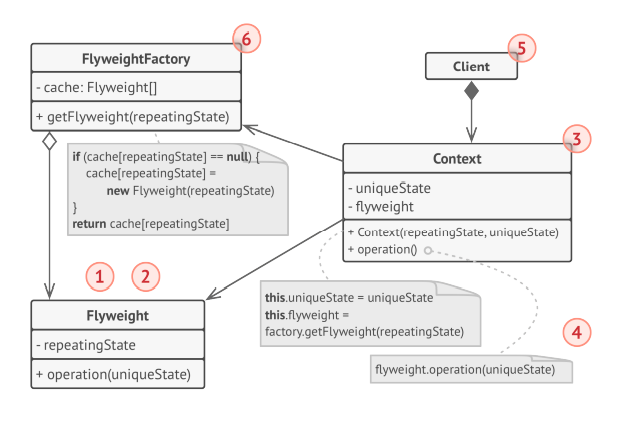
\includegraphics[scale=0.6]{image/structural/flyweight.png}
\end{center}
\begin{itemize}
    \item Về bản chất flyweight là gôm các điểm chung của các object thành 1 thành phần và kết hợp với các đối tượng sử dụng bộ đặc điểm chung đó.
\end{itemize}
\subsubsection{Ưu điểm và Nhược điểm}
Ta có các ưu nhược điểm sau:\\
Ưu điểm:
\begin{itemize}
    \item Tiết kiệm tài nguyên bộ nhớ bằng cách chia sẻ dữ liệu chung giữa các đối tượng.
    \item Giảm số lương đối tượng được tạo ra bằng cách chia sẻ đối tượng. Vì vậy tiết kiệm bộ nhớ và các thiết bị lưu trữ cần thiết.
\end{itemize}
Nhược điểm:
\begin{itemize}
    \item Cần quản lý sự chia sẻ dữ liệu một cách cẩn thận để đảm bảo tính toàn vẹn dữ liệu giữa các đối tượng.
    \item Việc chia sẻ dữ liệu có thể làm cho việc xử lý và quản lý phức tạp hơn.
\end{itemize}
\subsubsection{Code Example}
\begin{itemize}
    \item Ta có class Hình vuông và một nhà máy để tạo ra các hình vuông dựa vào vài yếu tố.
\end{itemize}
\begin{lstlisting}
#include <iostream>
#include <vector>
#include <map>

// Flyweight: Square
class Square {
private:
    std::string color;
    int size;

public:
    Square(const std::string& color, int size) : color(color), size(size) {}

    void draw(int x, int y) {
        std::cout << "Draw square: Color " << color << ", Size " << size << ", Position (" << x << ", " << y << ")" << std::endl;
    }
};

// Flyweight Factory: Manages shared Square objects
class SquareFactory {
private:
    std::map<std::string, Square*> squares;

public:
    Square* getSquare(const std::string& color, int size) {
        std::string key = color + "_" + std::to_string(size);
        if (squares.find(key) == squares.end()) {
            squares[key] = new Square(color, size);
        }
        return squares[key];
    }
};

// Client: Uses Square objects
int main() {
    SquareFactory squareFactory;

    std::vector<std::pair<int, int>> positions = { {0, 0}, {10, 5}, {3, 8}, {7, 2} };

    Square* blueSquare = squareFactory.getSquare("Blue", 10);
    Square* redSquare = squareFactory.getSquare("Red", 10);

    for (const auto& pos : positions) {
        blueSquare->draw(pos.first, pos.second);
        redSquare->draw(pos.first + 1, pos.second + 1);
    }

    return 0;
}

\end{lstlisting}
Ở hàm main, ta gọi một nhà máy sản xuất hình vuông và sản xuất 2 loại hình vuông xanh đỏ trên một bộ số có sẵn.\\
\newline
\textbf{Kết quả:}
\begin{lstlisting}
Draw square: Color Blue, Size 10, Position (0, 0)
Draw square: Color Red, Size 10, Position (1, 1)
Draw square: Color Blue, Size 10, Position (10, 5)
Draw square: Color Red, Size 10, Position (11, 6)
Draw square: Color Blue, Size 10, Position (3, 8)
Draw square: Color Red, Size 10, Position (4, 9)
Draw square: Color Blue, Size 10, Position (7, 2)
Draw square: Color Red, Size 10, Position (8, 3)
\end{lstlisting}
\subsubsection{Các Pattern liên quan}
\begin{itemize}
    \item Sử dụng các node lá của Composite nếu nó có thuộc tính cung có thể cài đặt theo kiểu Flyweight.
    \item Facade có thể kết hợp với Flyweight do flyweight là chia đối tượng lớn ra nhiều đối tượng nhỏ còn facade là gôm tất cả đối tượng nhỏ thành đối tượng lớn.
\end{itemize}
\subsection{Proxy}
\subsubsection{Định nghĩa}
Proxy là một mẫu thiết kế hướng đối tượng (design pattern) trong lập trình, thuộc nhóm mẫu cấu trúc (structural pattern). Nó cho phép bạn cung cấp một đối tượng trung gian (proxy) để kiểm soát quyền truy cập vào đối tượng thực (real object). Proxy hành động như một lớp ủy quyền và cung cấp một giao diện tương tự như đối tượng thực, cho phép kiểm soát và thực hiện các hoạt động bổ sung trước hoặc sau khi gọi đến đối tượng thực.
\subsubsection{Cách sử dụng}
Chúng ta có thể sử dụng proxy khi:
\begin{itemize}
    \item Khi bạn có một đối tượng dịch vụ nặng gây lãng phí tài nguyên hệ thống do luôn hoạt động, mặc dù thỉnh thoảng bạn chỉ cần nó.
    \item Khi bạn muốn chỉ những khách hàng cụ thể mới có thể sử dụng đối tượng dịch vụ.
    \item Khi bạn muốn che giấu thông tin về đối tượng thực khỏi người dùng, đặc biệt là trong trường hợp quyền truy cập hoặc bảo mật.
    \item Khi bạn muốn tạo ra các đối tượng khác nhau với chức năng tương tự, nhưng có quyền truy cập hoặc hành vi khác nhau.
\end{itemize}
\subsubsection{Cấu trúc}
\begin{itemize}
    \item Về lí thuyết, mẫu Proxy này tạo ra một class Proxy để ngắn cách người dùng truy cập trực tiếp vào đối tượng mà không thông qua lớp trung gian.
    \item Ở lớp Proxy này, ta có chứa cả đối tượng mà người dùng muốn truy cập.
\end{itemize}
Các thành phần chính của mẫu Proxy như sau:
\begin{itemize}
    \item ServiceInterface là một định nghĩa giao diện cho cả Proxy và Service để Proxy có thể được sử dụng bất kì nơi nào mà Service được mong đợi.
    \item Service là một class định nghĩa ServiceInterface mà Proxy đại diện.
    \item Proxy là một class có chứa một tham chiếu cho phép Proxy truy cập vào Service. 
\end{itemize}
\begin{center}
    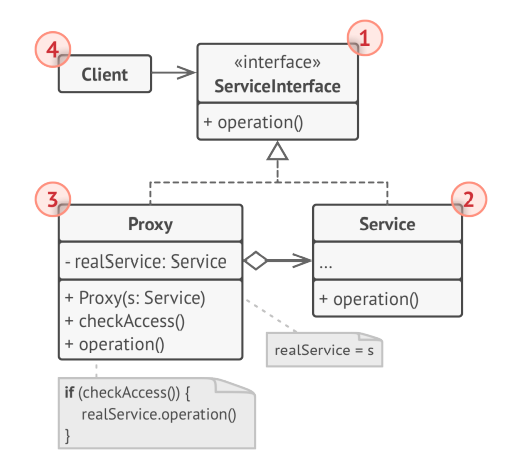
\includegraphics[scale=0.6]{image/structural/proxy.png}
\end{center}
\subsubsection{Ưu điểm và Nhược điểm}
Ta có các ưu nhược điểm sau:
Ưu điểm:
\begin{itemize}
    \item Proxy cho phép thêm các logic bổ sung mà không làm thay đổi đối tượng thực.
    \item Bảo vệ tính toàn vẹn của đối tượng thực bằng cách kiểm soát truy cập vào nó.
    \item Cung cấp một lớp trung gian để xử lý các yêu cầu phức tạp hoặc tốn nhiều tài nguyên của đối tượng thực.
\end{itemize}
Nhược điểm:
\begin{itemize}
    \item Tăng độ trễ trong việc gọi phương thức do cần thông qua lớp proxy.
\end{itemize}
\subsubsection{Code Example}
\begin{itemize}
    \item Ta có một ảnh thực, một ảnh proxy để kế thừa từ interface ảnh.
    \item Trong ảnh thực, ta có hàm trình bày và hàm tải từ đĩa.
    \item Ở cấu trúc trên, nếu chưa có ảnh nào được tải lên proxy thì lần truy cập đầu, proxy phải tải ảnh vào chỗ mình, các lần sau không cần thiết làm điều đó.
\end{itemize}
\begin{lstlisting}
#include <iostream>
#include <string>

// Common interface for the RealObject and Proxy
class Image {
public:
    virtual void display() = 0;
};

// RealObject
class RealImage : public Image {
private:
    std::string filename;

public:
    RealImage(const std::string& filename) : filename(filename) {
        loadFromDisk();
    }

    void display() override {
        std::cout << "Displaying image: " << filename << std::endl;
    }

    void loadFromDisk() {
        std::cout << "Loading image from disk: " << filename << std::endl;
    }
};

// Proxy
class ProxyImage : public Image {
private:
    std::string filename;
    RealImage* realImage;

public:
    ProxyImage(const std::string& filename) : filename(filename), realImage(nullptr) {}

    void display() override {
        if (realImage == nullptr) {
            realImage = new RealImage(filename);
        }
        realImage->display();
    }
};

int main() {
    // Use ProxyImage to create and display the image
    Image* image = new ProxyImage("image.jpg");

    // The first time displaying the image, it will load from disk
    image->display();

    // The second time displaying the image, it won't need to reload from disk
    image->display();

    delete image;

    return 0;
}


\end{lstlisting}
Ở hàm main, ta thực hiện tạo ảnh và display ảnh 2 lần. Ở lần đầu do phải tải ảnh lên proxy còn lần sau thì không cần thiết.\\
\newline
\textbf{Kết quả:}
\begin{lstlisting}
Loading image from disk: image.jpg
Displaying image: image.jpg
Displaying image: image.jpg
\end{lstlisting}
\subsubsection{Các Pattern liên quan}
\begin{itemize}
    \item Adapter để chuyển đổi các class còn Proxy tạo ra class để người dùng truy cập vào nó trước khi đụng được vào đối tượng thật. Chúng ta có thể kết hợp cả hai mẫu này như là để chuyển đổi giữa các Proxy.
    \item Decorator có cấu trúc giông với Proxy nhưng khác nhau về mục đích sử dụng. Decorator cho đối tượng thêm trách nhiệm còn Proxy thì kiểm soát quyền truy cập vào đối tượng.
\end{itemize}
\newpage
\section{Behavioral Pattern}
Ở phần Behavioral Patterns, ta có 10 mẫu Patterns cụ thể là \textbf{Chain of Responsibility}, \textbf{Command}, \textbf{Iterator}, \textbf{Mediator}, \textbf{Memento}, \textbf{Observer}, \textbf{State}, \textbf{Strategy}, \textbf{Template Method}, \textbf{Visitor}. Nhờ vào 10 mẫu này mà ta có các giải pháp để thực hiện hành vi của các đối tượng cũng như tương tác giữa các đối tượng với nhau để hoàn thành task được giao.\\
\subsection{Chain of Responsibility}
\subsubsection{Định nghĩa}
Chain of Responsibility là một mẫu thiết kế hành vi (behavioral design pattern) trong lập trình, nó cho phép một loạt các đối tượng xử lý một yêu cầu tuần tự. Yêu cầu được chuyển tiếp qua các đối tượng cho đến khi có một đối tượng trong chuỗi có thể xử lý yêu cầu đó hoặc khi không còn đối tượng nào có thể xử lý.
\subsubsection{Cách sử dụng}
Thông thương ở một số trường hợp sau ta hay sử dụng chain of responsibility:
\begin{itemize}
    \item Có nhiều hơn một đối tượng có khả thực xử lý một yêu cầu trong khi đối tượng cụ thể nào xử lý yêu cầu đó lại phụ thuộc vào ngữ cảnh sử dụng.
    \item Khi có nhiều đối tượng có thể xử lý một yêu cầu và bạn muốn cho phép các đối tượng này tự động chọn đối tượng xử lý thích hợp.
    \item Khi bạn muốn tạo ra một chuỗi linh hoạt và có thể thay đổi cấu trúc xử lý yêu cầu một cách động.
\end{itemize}
\subsubsection{Cấu trúc}
\begin{center}
    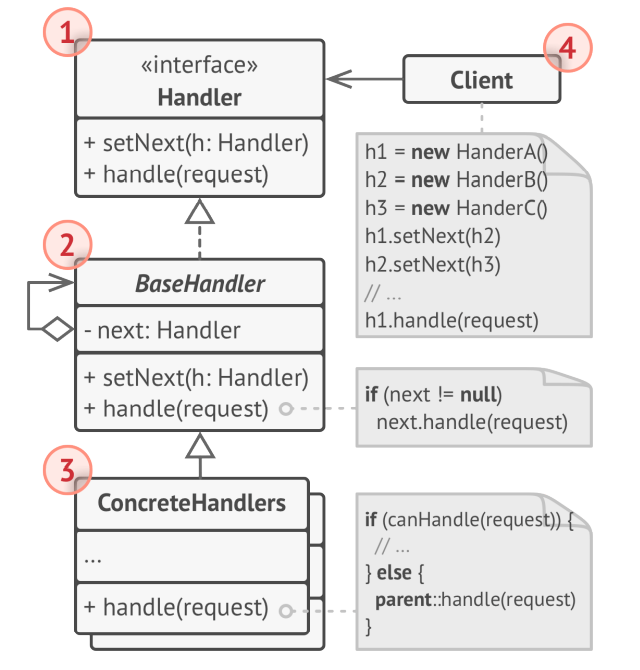
\includegraphics[scale= 0.45]{image/behavioral/cor.png}
\end{center}
\begin{itemize}
    \item Về cơ bản, cấu trúc này liên kết các class lại với nhau theo kiểu danh sách liên kết mỗi class này đều có hàm giải quyết vấn đề riêng của nó.
    \item Client sẽ sắp xếp thứ tự duyệt qua của các handlers.
\end{itemize}
Các thành phần chính:
\begin{itemize}
    \item Client là các dòng code ở trong main tạo ra các yêu cầu và yêu cầu đó sẽ được gửi đến các đối tượng tiếp nhận.
    \item Concrete Handler dùng để xử lí yêu cầu có con trỏ qua Concrete Handler khác nếu nó khong xử lí được.
    \item Handler là một interface hoặc abstract class có biến next.
    \item BaseHandler là một abstract class không bắt buộc có thể cài đặt các hàm chung cho chain of responsibility ở đây.
\end{itemize}
\subsubsection{Ưu điểm và Nhược điểm}
Ta có thể thấy tồn tại vài ưu nhược điểm sau
Ưu điểm:
\begin{itemize}
    \item Thay vì một đối tượng có khả năng xử lý yêu cầu chứa tham chiếu đến tất cả các đối tượng khác, nó chỉ cần một tham chiếu đến đối tượng tiếp theo. Tránh sự liên kết trực tiếp giữa đối tượng gửi yêu cầu (sender) và các đối tượng nhận yêu cầu (receivers).
    \item Dễ dàng thêm hoặc loại bỏ các bước xử lý trong chuỗi mà không ảnh hưởng đến các đối tượng khác.
\end{itemize}
Nhược điểm:
\begin{itemize}
    \item Một số yêu cầu có thể không được xử lý: Trường hợp tất cả Handler đều không xử lý
\end{itemize}
\subsubsection{Code Example}
\begin{itemize}
    \item Ta có một class Yêu cầu nâng cấp.
    \item Một loạt các class giải quyết yêu cầu nâng cấp có con trỏ chỉ đến bộ hanlder tiếp theo.
\end{itemize}
\begin{lstlisting}
#include <iostream>
#include <string>

class UpgradeRequest {
private:
    std::string component;
    std::string version;

public:
    UpgradeRequest(const std::string& component, const std::string& version)
        : component(component), version(version) {}

    std::string getComponent() const {
        return component;
    }

    std::string getVersion() const {
        return version;
    }
};

class UpgradeHandler {
protected:
    UpgradeHandler* nextHandler;

public:
    virtual void setNextHandler(UpgradeHandler* handler) {
        nextHandler = handler;
    }

    virtual void handleRequest(const UpgradeRequest& request) = 0;
};

class UIUpgradeHandler : public UpgradeHandler {
public:
    void handleRequest(const UpgradeRequest& request) override {
        if (request.getComponent() == "UI" && request.getVersion() == "2.0") {
            std::cout << "Upgrading UI component to version 2.0" << std::endl;
        } else if (nextHandler != nullptr) {
            nextHandler->handleRequest(request);
        } else {
            std::cout << "Upgrade request cannot be handled" << std::endl;
        }
    }
};

class DataUpgradeHandler : public UpgradeHandler {
public:
    void handleRequest(const UpgradeRequest& request) override {
        if (request.getComponent() == "Data" && request.getVersion() == "1.5") {
            std::cout << "Upgrading Data component to version 1.5" << std::endl;
        } else if (nextHandler != nullptr) {
            nextHandler->handleRequest(request);
        } else {
            std::cout << "Upgrade request cannot be handled" << std::endl;
        }
    }
};

class SecurityUpgradeHandler : public UpgradeHandler {
public:
    void handleRequest(const UpgradeRequest& request) override {
        if (request.getComponent() == "Security" && request.getVersion() == "3.2") {
            std::cout << "Upgrading Security component to version 3.2" << std::endl;
        } else if (nextHandler != nullptr) {
            nextHandler->handleRequest(request);
        } else {
            std::cout << "Upgrade request cannot be handled" << std::endl;
        }
    }
};

int main() {
    UpgradeHandler* uiUpgradeHandler = new UIUpgradeHandler();
    UpgradeHandler* dataUpgradeHandler = new DataUpgradeHandler();
    UpgradeHandler* securityUpgradeHandler = new SecurityUpgradeHandler();

    uiUpgradeHandler->setNextHandler(dataUpgradeHandler);
    dataUpgradeHandler->setNextHandler(securityUpgradeHandler);

    UpgradeRequest requestA("UI", "2.0");
    UpgradeRequest requestB("Data", "1.5");
    UpgradeRequest requestC("Security", "3.2");
    UpgradeRequest requestD("UI", "1.5");

    uiUpgradeHandler->handleRequest(requestA);
    uiUpgradeHandler->handleRequest(requestB);
    uiUpgradeHandler->handleRequest(requestC);
    uiUpgradeHandler->handleRequest(requestD);

    delete uiUpgradeHandler;
    delete dataUpgradeHandler;
    delete securityUpgradeHandler;

    return 0;
}

\end{lstlisting}
Ở hàm main, ta liên kết 3 hanlders lại với nhau. Ta có 4 yêu cầu từ khách hàng. Sau đó thực hiện giải quyết thì chỉ có duy nhất yêu cầu cuối cùng là không có bất cứ handler nào có thể giải quyết.\\
\newline
\textbf{Kết quả:}
\begin{lstlisting}
Upgrading UI component to version 2.0
Upgrading Data component to version 1.5
Upgrading Security component to version 3.2
Upgrade request cannot be handled
\end{lstlisting}
\subsubsection{Các Pattern liên quan}
\begin{itemize}
    \item Composite có thể được tích hợp chung. Ở trường hợp này các Leaf của CoR khi nhận yêu cầu sẽ được thực hiện tuần tự cho đến khi kết thúc.
    \item Có thể kết hợp với Command với các class Commands là các node lá của CoR và các command này sẽ được duyệt qua.
    \item Có thể kết hợp với Decorator bằng cách thêm thông tin vào các Leaf của CoR.
\end{itemize}

\subsection{Command}
\subsubsection{Định nghĩa}
Command là một mẫu thiết kế hành vi (behavioral design pattern) cho phép đóng gói các yêu cầu hoặc hành động vào một đối tượng riêng biệt. Nó chuyển đổi các yêu cầu thành một đối tượng độc lập, cho phép chúng ta thực hiện các yêu cầu, hàng loạt yêu cầu, hoặc hủy yêu cầu một cách linh hoạt.
\subsubsection{Cách sử dụng}
Thông thương, ta hay sử dụng mẫu thiết kế trên trong các trường hợp:
\begin{itemize}
    \item Khi bạn muốn tạo ra một hàng đợi các yêu cầu được thực thi theo thứ tự hoặc lưu trữ lịch sử các yêu cầu.
    \item Khi bạn muốn hỗ trợ hoạt động undo/redo.
    \item Phối hợp nhiều Command với nhau theo thứ tựtự.
\end{itemize}
\subsubsection{Cấu trúc}
\begin{center}
    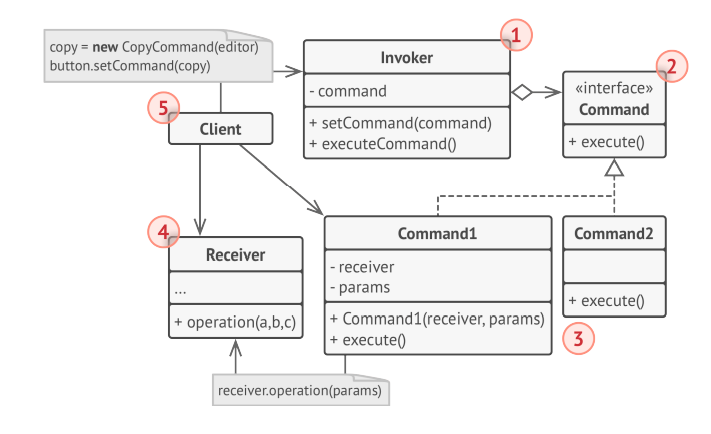
\includegraphics[scale= 0.6]{image/behavioral/command.png}
\end{center}
Các thành phần chính của mẫu:
\begin{itemize}
    \item Command là một interface hoặc abstract class chứa một phương thức thực thi, phương thức trừu tượng.
    \item ConcreteCommand là các subclass của Command định nghĩa operation.
    \item Invoker là một class tiếp nhận từ ConcreteCommand và gọi operation để thực thi.
    \item Receiver là một thành phần thực sử để xử lí cho case. Trong phương thức operation của ConcreteCommand chúng ta sẽ gọi method tương thích trong Receiver.
\end{itemize}
\subsubsection{Ưu điểm và Nhược điểm}
Có các ưu điểm và nhược điểm sau:
Ưu điểm:
\begin{itemize}
    \item Hỗ trợ các tính năng như undo/redo, quản lý lịch sử các yêu cầu.
    \item Giảm sự phụ thuộc giữa người gửi và người nhận yêu cầu.
\end{itemize}
Nhược điểm:
\begin{itemize}
    \item Có thể dẫn đến số lượng lớp lớn nếu có quá nhiều loại yêu cầu.
\end{itemize}

\subsubsection{Code Example}
\begin{itemize}
    \item Có một interface Command và 2 class LightOn và class LightOff được kế thừa.
    \item có class RemoteControl là Invoker có hàm excute để thực thi các lệnh.
\end{itemize}
\begin{lstlisting}
#include <iostream>
#include <string>
#include <vector>

// Command interface
class Command {
public:
    virtual void execute() = 0;
};

// Concrete command 1
class LightOnCommand : public Command {
private:
    std::string light;

public:
    LightOnCommand(const std::string& light) : light(light) {}

    void execute() override {
        std::cout << "Turn on " << light << " light" << std::endl;
    }
};

// Concrete command 2
class LightOffCommand : public Command {
private:
    std::string light;

public:
    LightOffCommand(const std::string& light) : light(light) {}

    void execute() override {
        std::cout << "Turn off " << light << " light" << std::endl;
    }
};

// Invoker
class RemoteControl {
private:
    std::vector<Command*> commands;

public:
    void setCommand(Command* command) {
        commands.push_back(command);
    }

    void executeCommands() {
        for (Command* command : commands) {
            command->execute();
        }
        commands.clear();
    }
};

int main() {
    // Create the invoker
    RemoteControl remote;

    // Create the commands
    Command* cmd1 = new LightOnCommand("Living Room");
    Command* cmd2 = new LightOnCommand("Bedroom");
    Command* cmd3 = new LightOffCommand("Bedroom");
    Command* cmd4 = new LightOffCommand("Living Room");

    // Set the commands
    remote.setCommand(cmd1);
    remote.setCommand(cmd2);
    remote.setCommand(cmd3);
    remote.setCommand(cmd4);

    // Execute the commands
    remote.executeCommands();

    // Clean up
    delete cmd1;
    delete cmd2;
    delete cmd3;
    delete cmd4;

    return 0;
}


\end{lstlisting}
Ở hàm main, ta tạo ra 4 lệnh, add nó vào remote rồi sau đó cho thực hiện cả 4 lệnh đó.\\
\newline
\textbf{Kết quả:}
\begin{lstlisting}
Turn on Living Room light
Turn on Bedroom light
Turn off Bedroom light
Turn off Living Room light
\end{lstlisting}
\subsubsection{Các Pattern liên quan}
\begin{itemize}
    \item CoR: nhận yêu cầu rôi thực hiện lần lượt các commands theo thứ tự.
    \item Mediator: thực hiện thông qua đối tượng gián tiếp.
    \item Observer: định nghĩa mối quan hệ một thay đổi các commands thay đổi theo.
\end{itemize}
\subsection{Iterator}
\subsubsection{Định nghĩa}
Iterator là một mẫu thiết kế hành vi (behavioral design pattern) cho phép truy cập tuần tự vào các phần tử của một tập hợp (collection) mà không tiết lộ cấu trúc nội bộ của nó. Nó cung cấp một cách tiếp cận thống nhất để duyệt qua các phần tử của một tập hợp mà không phụ thuộc vào kiểu cấu trúc dữ liệu của tập hợp đó.
\subsubsection{Cách sử dụng}
Ta sẽ sử dụng Pattern này trong các trường hợp:
\begin{itemize}
    \item Sử dụng mẫu Iterator khi collection của bạn có một cấu trúc dữ phức tạp, nhưng bạn muốn ẩn tính phức tạp chung của nó với các máy khác (để thuận tiện hoặc bảo mật).
    \item Khi được đặt trong logic kinh doanh của một ứng dụng, nó có thể làm lu mờ vai trò của source code gốc và làm cho nó khó bảo trì hơn. Với việc di chuyển source code đó đến các Iterator được chỉ định có thể giúp code của mình gọn gàng và sạch sẽ hơn.
    \item Sử dụng Iterator khi bạn muốn có một interface duy nhất để duyệt qua các phần tử của một tập hợp, code của mình có thể follow các cấu trúc dữ liệu khác nhau hoặc khi các loại cấu trúc chuỗi này chưa được biết trước.
\end{itemize}
\subsubsection{Cấu trúc}
\begin{center}
    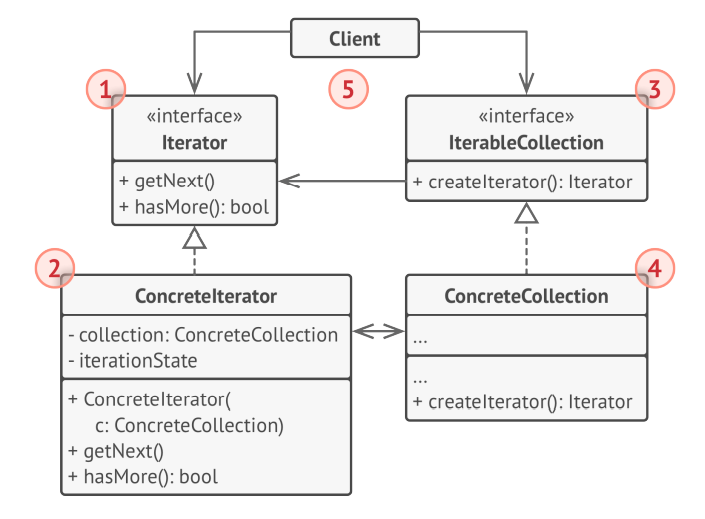
\includegraphics[scale= 0.6]{image/behavioral/iterator.png}
\end{center}
Các thành phần chính:
\begin{itemize}
    \item Một interface hay abstract class tên Iterator định nghĩa các hoạt động cần thiết.
    \item Concrete Iterator implement các phương thức trên.
    \item Collection Interface để khai báo một hoặc nhiều phương thức để nhận được các Iterator tương thích với collection.
    \item Concrete Collection trả về các phiên bản của một lớp Iterator cụ thể mỗi khi có các dòng code yêu cầu.
\end{itemize}
\subsubsection{Ưu điểm và Nhược điểm}
Có các ưu điểm và nhược điểm sau:
Ưu điểm:
\begin{itemize}
    \item Hỗ trợ nhiều cách duyệt qua các phần tử, bao gồm duyệt theo chiều thuận, chiều ngược và duyệt ngẫu nhiên.
    \item Chúng ta có thể truy cập song song trên cùng một tập hợp vì mỗi đối tượng iterator có chứa trạng thái riêng của nó.
\end{itemize}
Nhược điểm:
\begin{itemize}
    \item Sử dụng iterator có thể kém hiệu quả hơn so với việc duyệt qua các phần tử của bộ sưu tập một cách trực tiếp.
    \item Có thể không cần thiết nếu ứng dụng chỉ hoạt động với các collection đơn giản.
\end{itemize}
\subsubsection{Code Example}
\begin{itemize}
    \item Một interface Iterator và một VectorIterator là subclass.
\end{itemize}
\begin{lstlisting}
#include <iostream>
#include <vector>

// Iterator interface
class Iterator {
public:
    virtual bool hasNext() = 0;
    virtual int next() = 0;
};

// Concrete iterator
class VectorIterator : public Iterator {
private:
    std::vector<int>& vector;
    int index;

public:
    VectorIterator(std::vector<int>& vec) : vector(vec), index(0) {}

    bool hasNext() override {
        return index < vector.size();
    }

    int next() override {
        return vector[index++];
    }
};

// Client code
void printValues(Iterator& iterator) {
    while (iterator.hasNext()) {
        std::cout << iterator.next() << " ";
    }
    std::cout << std::endl;
}

int main() {
    std::vector<int> numbers = { 1, 2, 3, 4, 5 };
    VectorIterator iterator(numbers);

    printValues(iterator);

    return 0;
}

\end{lstlisting}
Ở hàm main, ta gọi một vector int là dùng iterator duyệt qua các giá trị đó.\\
\newline
\textbf{Kết quả:}
\begin{lstlisting}
1 2 3 4 5 
\end{lstlisting}
\subsubsection{Các Pattern liên quan}
\begin{itemize}
    \item Composite: ta thường dùng Iterator để duyệt qua cấu trúc cây.
    \item Memento: có thể kết hợp với Memento để lưu lại các trạng thái đã từng duyệt qua.
    \item Visitor: có thể kết hợp với Iterator để xem qua một cấu trúc dữ liệu phức tạp và thực hiện một số thao tác trên các phần tử của nó.
\end{itemize}

\subsection{Interpreter}
\subsubsection{Định nghĩa}
Interpreter là một mẫu Pattern thuộc Behavioral Pattern cung cấp giải pháp để tạo ra đối tượng dựa trên mô tả người dùng trong lúc hoạt động chương trình. Nó thực thi một dòng lệnh hoặc một khối lệnh một cách tuần tự tại thời điểm chạy chương trình. Interpreter thực thi các dòng lệnh bằng cách chuyển nó thành mã máy cho phép chạy ngay lặp tức.
\subsubsection{Cách sử dụng}
Thông thương, ta hay sử dụng mẫu thiết kế trên trong các trường hợp:
\begin{itemize}
    \item Cho phép lập trình viên phát triển và hiện thực mã lệnh nhanh mà không cần phải complie. Sau mỗi lần chỉnh sửa mã nguồn, lập trình viên có thể chạy và xem kết quả ngay lặp tức.
    \item  Interpreter thường được sử dụng cho các ngôn ngữ có cấu trúc chạy từ trên xuống dưới như Python, Javascript,...
\end{itemize}
\subsubsection{Cấu trúc}
\begin{center}
    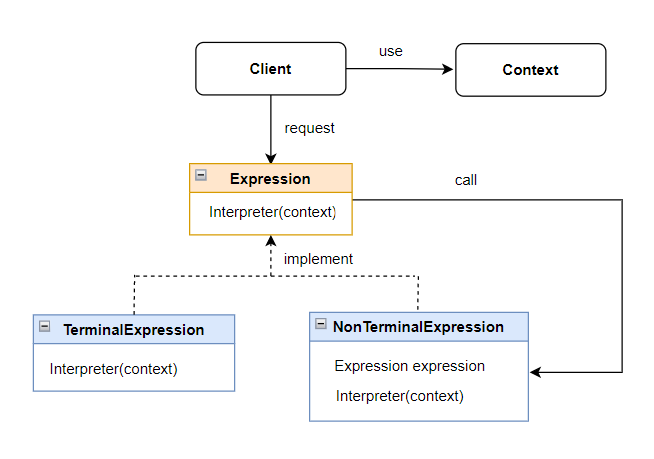
\includegraphics[scale= 0.6]{image/behavioral/interpreter.png}
\end{center}
Các thành phần chính của mẫu:
\begin{itemize}
    \item AbstractionExpression là một Class khai báo một giao diện cho việc thực thi một thao tác bất kì.
    \item TerminalExpression là một class cài đặt một thao tác thông dịch liên kết với những ký pháp đầu cuối, đóng vai trò một thể nghiệm được yêu cầu cho mọi ký pháp đầu cuối trong câu.
    \item NonterminalExpression là một class có thể chứa TerminalExpression bên trong và cũng có thể chứa một NonterminalExpression khác. Nó đóng vai trò như là “ngữ pháp” của ngôn ngữ đặc tả.
    \item Context: Là đối tượng thông tin để thực hiện thông dịch. Đối tượng này là toàn cục đối với quá trình thông dịch.
\end{itemize}
\subsubsection{Ưu điểm và Nhược điểm}
Có các ưu điểm và nhược điểm sau:
Ưu điểm:
\begin{itemize}
    \item Giảm số lượng những lớp con không cần thiết.
    \item Cho phép ẩn các chi tiết implement từ client.
    \item Vì không cần biên dịch trước, việc chỉnh sửa và chạy lại mã nguồn nhanh chóng.
    \item Interpreter có thể chạy trên nhiều nền tảng khác nhau mà không cần biên dịch lại.
\end{itemize}
Nhược điểm:
\begin{itemize}
    \item Interpreter phải dịch và thực thi từng dòng lệnh một tại thời điểm chạy, do đó tốn thời gian hơn so với việc biên dịch trước.
    \item Hiệu suất thấp.
    \item Đòi hỏi ngôn ngữ được xây dựng phải có cấu trúc đơn giản.
\end{itemize}

\subsubsection{Code Example}
\begin{itemize}
    \item Có một abtract class Expression để địng nghĩa dạng của kiểu lưu Expression.
    \item Các class Variable, Constant, Add, Subtract đại diện cho các biểu thức đại số (terminal và non-terminal) được kế thừa từ lớp Expresion ở trên.
\end{itemize}
\begin{lstlisting}
#include <iostream>
#include <string>
#include <unordered_map>

// Abstract Expression
class Expression {
public:
    virtual int interpret(std::unordered_map<char, int>& variables) = 0;
};

// Terminal Expression
class Variable : public Expression {
private:
    char variableName;
public:
    Variable(char name) : variableName(name) {}
    int interpret(std::unordered_map<char, int>& variables) override {
        return variables[variableName];
    }
};

// Terminal Expression
class Constant : public Expression {
private:
    int value;
public:
    Constant(int val) : value(val) {}
    int interpret(std::unordered_map<char, int>& variables) override {
        return value;
    }
};

// Non-terminal Expression
class Add : public Expression {
private:
    Expression* left;
    Expression* right;
public:
    Add(Expression* l, Expression* r) : left(l), right(r) {}
    int interpret(std::unordered_map<char, int>& variables) override {
        return left->interpret(variables) + right->interpret(variables);
    }
};

// Non-terminal Expression
class Subtract : public Expression {
private:
    Expression* left;
    Expression* right;
public:
    Subtract(Expression* l, Expression* r) : left(l), right(r) {}
    int interpret(std::unordered_map<char, int>& variables) override {
        return left->interpret(variables) - right->interpret(variables);
    }
};

// Client
int main() {
    std::unordered_map<char, int> variables;
    variables['x'] = 5;
    variables['y'] = 3;

    Expression* expression = new Subtract(
        new Add(new Variable('x'), new Variable('y')),
        new Constant(2)
    );

    int result = expression->interpret(variables);
    std::cout << "Result: " << result << std::endl;

    delete expression;

    return 0;
}


\end{lstlisting}
Trong phần main(), chúng ta khởi tạo các biến và xây dựng một biểu thức để tính toán (x + y - 2). Sau đó, chúng ta gọi hàm interpret() của biểu thức đó với một unorderedmap chứa giá trị của các biến (x = 5 và y = 3). Kết quả tính toán được in ra màn hình.
\\
\newline
\textbf{Kết quả:}
\begin{lstlisting}
Result: 6
\end{lstlisting}
\subsubsection{Các Pattern liên quan}
\begin{itemize}
    \item Composite là cây có trúc ngữ pháp trừu tượng
    \item Sử dụng Iterator để duyệt các dòng lệnh.
    \item Visitor có thể được sử dụng để duy trì hành vi trên mỗi nút trong cây cú pháp trừu tượng của lớp.
\end{itemize}
\subsection{Mediator}
\subsubsection{Định nghĩa}
Mediator là một mẫu thiết kế hành vi (behavioral design pattern) cho phép giảm sự phụ thuộc giữa các đối tượng và tạo một sự tương tác trung gian giữa chúng thông qua một đối tượng trung tâm được gọi là Mediator. Mediator đóng vai trò làm trung gian, điều phối và quản lý tất cả các tương tác giữa các đối tượng thành phần.
\subsubsection{Cách sử dụng}
Trong vài trường hợp sau, ta có thể áp dụng Pattern này vào:
\begin{itemize}
    \item Khi sự phụ thuộc giữa các đối tượng dẫn đến một hệ thống phức tạp và khó khăn trong việc bảo trì và mở rộng.
    \item Sử dụng khi tập hợp các đối tượng giao tiếp theo những cách thức được xác định rõ ràng nhưng cách thức đó quá phức tạp.
    \item Khi bạn muốn tạo một sự tương tác trung gian giữa các đối tượng mà không làm cho chúng gắn kết với nhau.
\end{itemize}
\subsubsection{Cấu trúc}
\begin{center}
    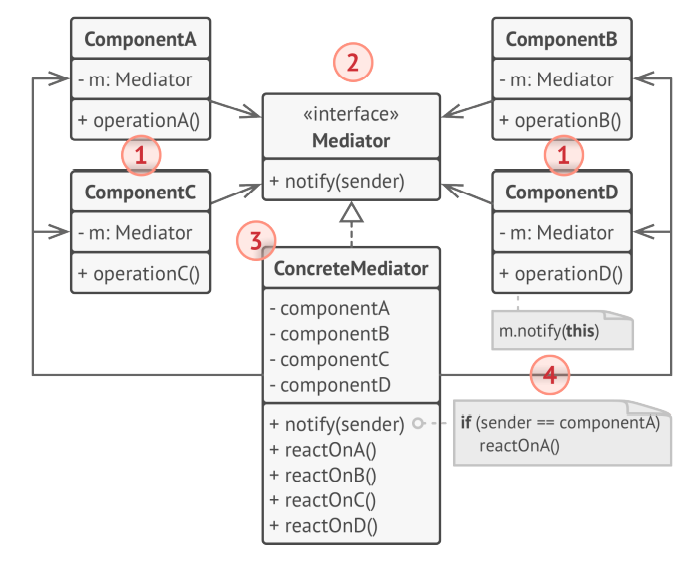
\includegraphics[scale=0.6]{image/behavioral/mediator.png}
\end{center}
\subsubsection{Ưu điểm và Nhược điểm}
Có các ưu điểm và nhược điểm sau:
Ưu điểm:
\begin{itemize}
    \item Đơn giản hóa cách giao tiếp giữa các đối tượng, Một Mediator sẽ thay thế mối quan hệ nhiều nhiều (many-to-many) giữa các component bằng quan hệ một-nhiều (one-to-many) giữa một mediator với các component.
    \item Quản lý tập trung, giúp làm rõ các component tương tác trong hệ thống như thế nào trong hệ thống.
    \item Giảm sự phụ thuộc giữa các đối tượng, làm cho hệ thống linh hoạt hơn và dễ dàng mở rộng.
    \item Tách biệt logic điều phối và logic của các đối tượng thành phần, làm cho mã dễ đọc và bảo trì hơn.
\end{itemize}
Nhược điểm:
\begin{itemize}
    \item Mediator có thể trở thành một điểm trung tâm phụ thuộc, làm giảm tính độc lập và sự tái sử dụng của các đối tượng thành phần.
\end{itemize}
\subsubsection{Code Example}
\begin{itemize}
    \item Có một interface Colleague và class User là subclass.
    \item Có một interface Mediator và class ChatRoom là subclass.
\end{itemize}
\begin{lstlisting}
#include <iostream>
#include <string>
#include <vector>

// Forward declaration
class Colleague;

// Mediator
class Mediator {
public:
    virtual void sendMessage(Colleague* sender, const std::string& message) = 0;
};

// Colleague (Abstract Base Class)
class Colleague {
protected:
    Mediator* mediator;

public:
    explicit Colleague(Mediator* mediator) : mediator(mediator) {}

    virtual void receiveMessage(const std::string& message) = 0;
    virtual void sendMessage(const std::string& message) = 0;
};

// Concrete Colleague
class User : public Colleague {
private:
    std::string name;

public:
    User(const std::string& name, Mediator* mediator) : name(name), Colleague(mediator) {}

    void receiveMessage(const std::string& message) override {
        std::cout << name << " received message: " << message << std::endl;
    }

    void sendMessage(const std::string& message) override {
        mediator->sendMessage(this, message);
    }
};

// Concrete Mediator
class ChatRoom : public Mediator {
private:
    std::vector<User*> users;

public:
    void addUser(User* user) {
        users.push_back(user);
    }

    void sendMessage(Colleague* sender, const std::string& message) override {
        for (auto user : users) {
            if (user != sender) {
                user->receiveMessage(message);
            }
        }
    }
};

int main() {
    ChatRoom chatRoom;

    User user1("Alice", &chatRoom);
    User user2("Bob", &chatRoom);
    User user3("Charlie", &chatRoom);

    chatRoom.addUser(&user1);
    chatRoom.addUser(&user2);
    chatRoom.addUser(&user3);

    user1.sendMessage("Hello, everyone!");
    user2.sendMessage("Hi, Alice!");

    return 0;
}

\end{lstlisting}
Ở hàm main, ta gọi 3 user cho vào chatRoom và thực hiện việc gửi tin nhắn.\\
\newline
\textbf{Kết quả:}
\begin{lstlisting}
Bob received message: Hello, everyone!
Charlie received message: Hello, everyone!
Alice received message: Hi, Alice!
Charlie received message: Hi, Alice!
\end{lstlisting}
\subsubsection{Các Pattern liên quan}
\begin{itemize}
    \item Chain of Responsibility truyền request lần lượt chứa các receiver tiềm năng cho đến khi có receiver thích hợp có thể giải quyết được. Command thì tạo ra các kết nối một chiều giữa các receiver và các sender.
    \item Mediator loại bỏ các kết nối trực tiếp giữa các receiver và các sender rồi bắt buộc chúng phải giao tiếp không trực tiếp thông qua đối tượng mediator.
    \item Observer cho phép các receiver chủ động trong việc subscribe và unsubscribe receiving requests.
    \item Facade thì định nghĩa một interface được đơn giản hóa đến các đối tượng của hệ thống con nhưng nó không tạo thêm các chức năng mới.
    \item Mediator thì sẽ trung gian hóa sự giao tiếp giữa các component trong hệ thống.
\end{itemize}
\subsection{Memento}
\subsubsection{Định nghĩa}
Memento là một mẫu thiết kế hành vi trong đó một đối tượng được tạo ra để lưu trữ trạng thái của một đối tượng khác và khôi phục lại trạng thái đó sau này mà không tiết lộ chi tiết cài đặt.
\subsubsection{Cách sử dụng}
Memento được sử dụng khi bạn muốn lưu trữ trạng thái của một đối tượng và khôi phục lại trạng thái đó sau này. Điều này có thể xảy ra trong các tình huống như:
\begin{itemize}
    \item Khi bạn muốn lưu trữ một checkpoint hoặc trạng thái tạm thời của một ứng dụng để có thể hoàn tác hoặc khôi phục lại trạng thái trước đó.
    \item Khi bạn muốn theo dõi và lưu lại lịch sử của một đối tượng để có thể quay lại các trạng thái trước đó.
\end{itemize}
\subsubsection{Cấu trúc}
\begin{center}
    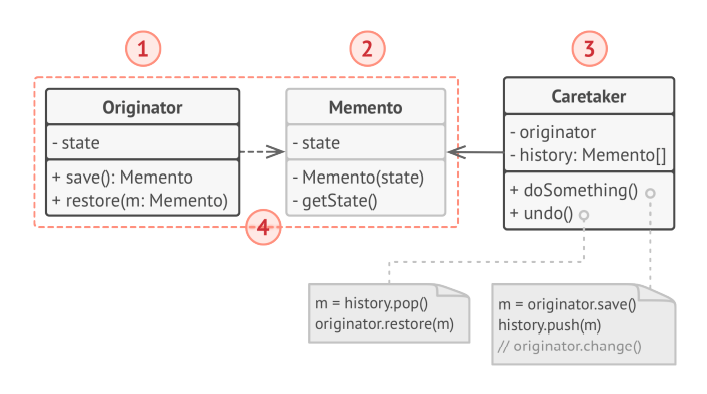
\includegraphics[scale = 0.6]{image/behavioral/memento.png}
\end{center}
\subsubsection{Ưu điểm và Nhược điểm}
Có các ưu điểm và nhược điểm sau:
Ưu điểm:
\begin{itemize}
    \item Nguyên tắc đơn trách nhiệm: Memento chỉ tương tác với nguồn gốc của nó và không gây phụ thuộc đối tượng khác.
    \item Bảo vệ dữ liệu: Dữ liệu bên trong Memento không thể truy cập hoặc sửa đổi từ bên ngoài.
    \item Khi có một số lượng lớn Memento được tạo ra có thể gặp vấn đề về bộ nhớ, performance của ứng dụng.
\end{itemize}
Nhược điểm:
\begin{itemize}
    \item Dùng quá nhiều bộ nhớ: Nếu Memento lưu trữ nhiều trạng thái hoặc đối tượng lớn, nó có thể tiêu tốn nhiều bộ nhớ.
    \item Hiệu suất: Nếu việc tạo và khôi phục Memento quá tốn kém và ảnh hưởng đến hiệu suất chung của ứng dụng.
\end{itemize}
\subsubsection{Code Example}
\begin{itemize}
    \item Có một class Memento chứa level và score.
    \item Một class Game có các phương thức và phải có hàm saveState để giữ trạng thái hiện tại.
    \item Class GameHistory lưu các memento của game.
\end{itemize}
\begin{lstlisting}
#include <iostream>
#include <vector>

// Memento: Represents the snapshot of the state
class Memento {
private:
    int level;
    int score;

public:
    Memento(int level, int score) : level(level), score(score) {}

    int getLevel() const {
        return level;
    }

    int getScore() const {
        return score;
    }
};

// Originator: Creates and restores from mementos
class Game {
private:
    int level;
    int score;

public:
    void playLevel(int level) {
        this->level = level;
        score = 0;
        std::cout << "Playing Level " << level << std::endl;
    }

    void increaseScore(int points) {
        score += points;
        std::cout << "Score increased by " << points << ". Current score: " << score << std::endl;
    }

    Memento saveState() const {
        return Memento(level, score);
    }

    void restoreState(const Memento& memento) {
        level = memento.getLevel();
        score = memento.getScore();
        std::cout << "Restored state: Level " << level << ", Score " << score << std::endl;
    }
};

// Caretaker: Manages the mementos
class GameHistory {
private:
    std::vector<Memento> mementos;

public:
    void addMemento(const Memento& memento) {
        mementos.push_back(memento);
    }

    Memento getMemento(int index) const {
        return mementos[index];
    }
};

int main() {
    Game game;
    GameHistory history;

    // Play Level 1
    game.playLevel(1);
    game.increaseScore(100);
    history.addMemento(game.saveState());

    // Play Level 2
    game.playLevel(2);
    game.increaseScore(150);
    history.addMemento(game.saveState());

    // Play Level 3
    game.playLevel(3);
    game.increaseScore(200);

    // Restore state from Level 2
    game.restoreState(history.getMemento(1));

    return 0;
}

\end{lstlisting}
Ở hàm main, ta thực hiện chơi 3 màn và restore lại màn 2.\\
\newline
\textbf{Kết quả:}
\begin{lstlisting}
Playing Level 1
Score increased by 100. Current score: 100
Playing Level 2
Score increased by 150. Current score: 150
Playing Level 3
Score increased by 200. Current score: 200
Restored state: Level 2, Score 150
\end{lstlisting}
\subsubsection{Các Pattern liên quan}
\begin{itemize}
    \item Két hợp với Command để thực hiện các lệnh hoàn tác.
    \item Kết hợp với Iterator để nắm bắt các trạng thái và thực hiên các lệnh khôi phục.
    \item Hoặc đơn giản chỉ cần ở thời điểm nào đó tạo Clone rồi thời điểm khác lại tạo Clone là ta đã có Memento bản thu nhỏ.
\end{itemize}
\subsection{Observer}
\subsubsection{Định nghĩa}
Observer là một mẫu thiết kế hành vi trong đó có một đối tượng chủ đạo (subject) duy trì danh sách các đối tượng quan sát (observers) và thông báo cho chúng về bất kỳ sự thay đổi nào trong trạng thái của nó. Điều này cho phép các đối tượng quan sát tự động cập nhật khi có sự thay đổi xảy ra.
\subsubsection{Cách sử dụng}
Ta sẽ sử dụng mẫu Pattern trên trong các trường hợp sau:
\begin{itemize}
    \item Sự thay đổi trạng thái ở 1 đối tượng cần được thông báo đến các đối tượng khác mà không phải giữ chúng liên kết quá chặt chẽ.
    \item Khi thay đổi một đối tượng yêu cầu việc thay đổi đến các đối tượng khác, và bạn không biết số lượng đối tượng cần thay đổi.
    \item Khi bạn muốn giảm sự phụ thuộc giữa các đối tượng và cho phép chúng hoạt động độc lập với nhau.
\end{itemize}
\subsubsection{Cấu trúc}
\begin{center}
    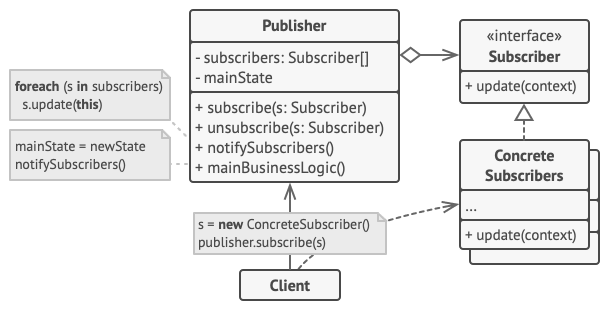
\includegraphics[scale= 0.6]{image/behavioral/observer.png}
\end{center}
\subsubsection{Ưu điểm và Nhược điểm}
Có các ưu điểm và nhược điểm sau:
Ưu điểm:
\begin{itemize}
    \item Sự thay đổi trạng thái ở 1 đối tượng có thể được thông báo đến các đối tượng khác mà không phải giữ chúng liên kết quá chặt chẽ.
    \item Không giới hạn số lượng Observer
    \item Đảm bảo sự tương tác giữa các đối tượng không phụ thuộc: Subject và observers không biết gì về sự tồn tại của nhau, do đó, chúng có thể hoạt động một cách độc lập và tái sử dụng được.
\end{itemize}
Nhược điểm:
\begin{itemize}
    \item Khi có nhiều observers và có nhiều thông báo được gửi đi, quá trình thông báo có thể gây ra sự chậm trễ và ảnh hưởng đến hiệu năng của hệ thống.
    \item Bởi vì các Observer không biết về sự hiện diện của nhau, nó có thể gây tốn nhiều chi phí của việc thay đổi Subject.
\end{itemize}
\subsubsection{Code Example}
\begin{itemize}
    \item Có interface Observer, Display là subclass có hàm update để cập nhật trạng thái.
    \item Có class WeatherStation.
\end{itemize}
\begin{lstlisting}
#include <iostream>
#include <vector>
#include <algorithm>

// Observer interface
class Observer {
public:
    virtual void update(int temperature) = 0;
};

// Subject class
class WeatherStation {
private:
    int temperature;
    std::vector<Observer*> observers;

public:
    void attach(Observer* observer) {
        observers.push_back(observer);
    }

    void detach(Observer* observer) {
        auto it = std::find(observers.begin(), observers.end(), observer);
        if (it != observers.end()) {
            observers.erase(it);
        }
    }

    void setTemperature(int newTemperature) {
        temperature = newTemperature;
        notify();
    }

    void notify() {
        for (auto observer : observers) {
            observer->update(temperature);
        }
    }
};

// Concrete Observer class
class Display : public Observer {
public:
    void update(int temperature) {
        std::cout << "Temperature changed: " << temperature << std::endl;
    }
};

int main() {
    // Create weather station and displays
    WeatherStation weatherStation;
    Display display1;
    Display display2;

    // Attach displays to the weather station
    weatherStation.attach(&display1);
    weatherStation.attach(&display2);

    // Set the temperature in the weather station
    weatherStation.setTemperature(25);

    // Detach one display from the weather station
    weatherStation.detach(&display1);

    // Set another temperature in the weather station
    weatherStation.setTemperature(30);

    // Attach display1 back to the weather station
    weatherStation.attach(&display1);

    // Set a third temperature in the weather station
    weatherStation.setTemperature(35);

    return 0;
}


\end{lstlisting}
Ở hàm main, ta tạo 2 display và lần lượt gán cho weatherStation đó với 2 loại Display. Sau đó, điều chỉnh nhiệt độ. Rồi bỏ đi một display trong weatherStation rồi lại điều chỉnh nhiệt độ. Xong lại thêm vào lại và điều chỉnh nhiệt đọ.\\
\newline
\textbf{Kết quả:}
\begin{lstlisting}
Temperature changed: 25
Temperature changed: 25
Temperature changed: 30
Temperature changed: 35
Temperature changed: 35
\end{lstlisting}
\subsubsection{Các Pattern liên quan}
\begin{itemize}
    \item Chain of Responsibility: duyệt theo thứ tự.
    \item Command: thiết kế mối quan hệ một chiều giữa người gửi và nhận.
    \item Mediator: dùng để loại bỏ kết nối trực tiếp giữa người gửi và nhận. 
    \item Observer: cho phép người nhận đăng kí động và hủy nhận yêu cầu.
\end{itemize}

\subsection{State}
\subsubsection{Định nghĩa}
State Pattern là một mẫu thiết kế thuộc nhóm Behavioral Pattern. State Pattern là một mẫu thiết kế hành vi cho phép một object thay đổi hành vi của nó khi trạng thái bên trong của nó thay đổi.
\subsubsection{Cách sử dụng}
Ta có thể sử dụng State Pattern trong các trường hợp sau:
\begin{itemize}
    \item Khi bạn có một object hoạt động khác nhau tùy thuộc vào trạng thái hiện tại của nó, số lượng trạng thái là rất lớn và code của trạng thái cụ thể thường xuyên thay đổi.
    \item Khi không muốn sử dụng nhiều câu lệnh điều kiện (if-else hoặc switch-case) để kiểm tra trạng thái của đối tượng.
    \item Khi bạn có nhiều code trùng lặp qua các trạng thái và chuyển đổi tương tự của State Pattern dựa trên điều kiện.
\end{itemize}
\subsubsection{Cấu trúc}
\begin{center}
    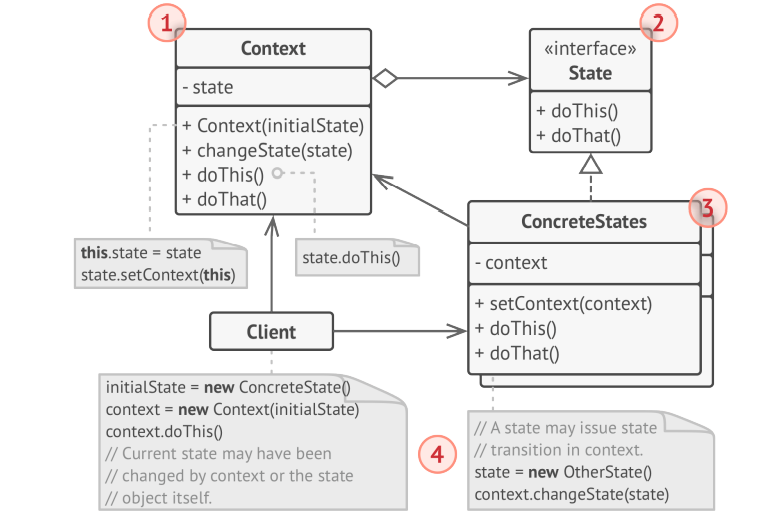
\includegraphics[scale=0.6]{image/behavioral/state.png}
\end{center}
\subsubsection{Ưu điểm và Nhược điểm}
Ta có rất nhiều ưu nhược điểm như sau:\\\\
Ưu điểm:
\begin{itemize}
    \item Mẫu State cho phép mô hình hóa trực quan các trạng thái khác nhau và cách chúng tương tác với nhau.
    \item Thay vì sử dụng nhiều câu lệnh điều kiện, mẫu State giúp tách biệt logic của từng trạng thái thành các lớp riêng biệt, giảm sự phức tạp của mã.
\end{itemize}
Nhược điểm:
\begin{itemize}
    \item Mẫu State có thể tạo ra nhiều lớp con để đại diện cho từng trạng thái, dẫn đến việc tăng số lượng lớp trong mã nguồn.
    \item Logic của mỗi trạng thái có thể phân mảnh trong các lớp con khác nhau, làm cho mã nguồn khó hiểu và duy trì.
\end{itemize}
\subsubsection{Code Example}
\begin{itemize}
    \item Có các class State con.
    \item Một các Context chữa State hiện tại.
\end{itemize}
\begin{lstlisting}
#include <iostream>

// State interface
class State {
public:
    virtual void handleState() = 0;
};

// Concrete states
class ConcreteStateA : public State {
public:
    void handleState() override {
        std::cout << "Handling state A." << std::endl;
    }
};

class ConcreteStateB : public State {
public:
    void handleState() override {
        std::cout << "Handling state B." << std::endl;
    }
};

// Context class
class Context {
private:
    State* currentState;

public:
    Context() {
        currentState = nullptr;
    }

    void setState(State* state) {
        currentState = state;
    }

    void request() {
        if (currentState) {
            currentState->handleState();
        }
    }
};

int main() {
    Context context;

    // Set initial state to A
    ConcreteStateA stateA;
    context.setState(&stateA);
    context.request();

    // Change state to B
    ConcreteStateB stateB;
    context.setState(&stateB);
    context.request();

    return 0;
}

\end{lstlisting}
Ở hàm main, Ta tạo 2 state r set State cho context r request nó sau đó chuyển context qua state khác rồi request nó.\\
\newline
\textbf{Kết quả:}
\begin{lstlisting}
Handling state A.
Handling state B.
\end{lstlisting}
\subsubsection{Các Pattern liên quan}
\begin{itemize}
    \item Bridge, State, Strategy có cấu trúc rất giống nhau. Tuy nhiên, chúng đều giải quyết các vấn đề khác nhau.
    \item State là bản mở rộng của Strategy. Cả hai Pattern đều dựa trên thành phần: chúng thay đổi hành vi của ngữ cảnh bằng cách ủy quyền một số công việc cho các object trợ giúp.
    \item Gần giống strategy, chuyển đổi các chiến lược thông qua các phương thức được định nghĩa trong interface. State không hạn chế sự phụ thuộc giữa các trạng thái cụ thể, cho phép chúng thay đổi trạng thái của ngữ cảnh theo ý muốn.
\end{itemize}



\subsection{Strategy}
\subsubsection{Định nghĩa}
Strategy (Chiến lược) là một mẫu thiết kế hành vi cho phép đối tượng thay đổi thuật toán được sử dụng trong quá trình thực thi một hành động cụ thể mà không ảnh hưởng đến các đối tượng khác hoặc cấu trúc của chúng. Mẫu này tách rời thuật toán khỏi đối tượng sử dụng nó, giúp tăng tính linh hoạt và tái sử dụng trong việc áp dụng các thuật toán khác nhau.
\subsubsection{Cách sử dụng}
Ta có thể sử dụng Strategy Pattern trong các trường hợp sau:
\begin{itemize}
    \item Khi có một hành động cần thực hiện, nhưng có nhiều thuật toán khác nhau có thể được áp dụng, và cần linh hoạt trong việc chọn thuật toán tại thời điểm chạy.
    \item Khi muốn tránh sự phức tạp của việc sử dụng nhiều câu lệnh điều kiện (if-else hoặc switch-case) để chọn thuật toán.
    \item Khi muốn tránh sự phức tạp của việc sử dụng nhiều câu lệnh điều kiện (if-else hoặc switch-case) để chọn thuật toán.
\end{itemize}
\subsubsection{Cấu trúc}
\begin{center}
    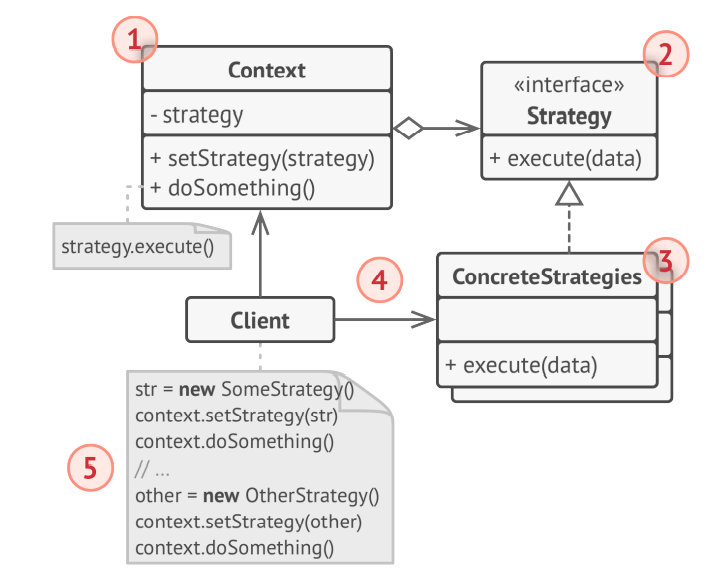
\includegraphics[scale=0.6]{image/behavioral/strategy.png}
\end{center}
\subsubsection{Ưu điểm và Nhược điểm}
Ta có rất nhiều ưu nhược điểm như sau:\\\\
Ưu điểm:
\begin{itemize}
    \item Linh hoạt và dễ dàng thay đổi thuật toán tại thời điểm chạy.
    \item Khi thay đổi thuật toán hoặc khi thêm mới thuật toán, không cần thay đổi code phần context.
    \item Có thể thay thế việc kế thừa bằng việc encapsulate thuật toán.
\end{itemize}
Nhược điểm:
\begin{itemize}
    \item Tăng số lượng các lớp và đối tượng, đặc biệt khi có nhiều thuật toán khác nhau.
    \item Cần phải hiểu rõ các thuật toán khác nhau để chọn và sử dụng một cách phù hợp.
\end{itemize}
\subsubsection{Code Example}
\begin{itemize}
    \item Có một interface và 2 concrete class thực hiện hóa 2 hàm sort.
    \item Một class Sorter có Strategy sort trong đó.
\end{itemize}
\begin{lstlisting}
#include <iostream>

// Strategy interface
class SortingStrategy {
public:
    virtual void sort(int* arr, int size) = 0;
};

// Concrete strategies
class QuickSortStrategy : public SortingStrategy {
public:
    void sort(int* arr, int size) override {
        std::cout << "Sorting using Quick Sort." << std::endl;
        // Perform Quick Sort algorithm
    }
};

class MergeSortStrategy : public SortingStrategy {
public:
    void sort(int* arr, int size) override {
        std::cout << "Sorting using Merge Sort." << std::endl;
        // Perform Merge Sort algorithm
    }
};

// Context class
class Sorter {
private:
    SortingStrategy* strategy;

public:
    void setStrategy(SortingStrategy* sortingStrategy) {
        strategy = sortingStrategy;
    }

    void sortArray(int* arr, int size) {
        strategy->sort(arr, size);
    }
};

int main() {
    int arr[] = {5, 2, 8, 1, 9};
    int size = sizeof(arr) / sizeof(arr[0]);

    Sorter sorter;

    QuickSortStrategy quickSortStrategy;
    MergeSortStrategy mergeSortStrategy;

    sorter.setStrategy(&quickSortStrategy);
    sorter.sortArray(arr, size);

    sorter.setStrategy(&mergeSortStrategy);
    sorter.sortArray(arr, size);

    return 0;
}

\end{lstlisting}
Ở hàm main, ta tạo ra 2 kiểu sort rồi thực hiện tuần tự 2 loại sort.\\
\newline
\textbf{Kết quả:}
\begin{lstlisting}
Sorting using Quick Sort.
Sorting using Merge Sort.
\end{lstlisting}
\subsubsection{Các Pattern liên quan}
\begin{itemize}
    \item Bridge có cấu trúc gống Strategy dựa trên composition.
    \item Command: giống nhau ở chỗ tham số hóa một đối tượng và hành động.
    \item State: là một bản mở rộng của Strategy.
\end{itemize}
\subsection{Template Method}
\subsubsection{Định nghĩa}
Template Method (Phương pháp mẫu) là một mẫu thiết kế hành vi cho phép định nghĩa một bản thiết kế mẫu cho một thuật toán và để các bước cụ thể của thuật toán được triển khai bởi các lớp con. Mẫu này xác định một khung (template) cho quy trình thực hiện một nhiệm vụ, trong đó một số bước được định nghĩa trong lớp gốc và các bước khác được chuyển giao cho các lớp con để triển khai.
\subsubsection{Cách sử dụng}
Ta có thể sử dụng Template Method Pattern trong các trường hợp sau:
\begin{itemize}
    \item Khi có một thuật toán với nhiều bước và mong muốn cho phép tùy chỉnh chúng trong lớp con.
    \item Mong muốn chỉ có một triển khai phương thức trừu tượng duy nhất của một thuật toán.
    \item Khi có một thuật toán chung, nhưng các bước cụ thể của thuật toán có thể thay đổi hoặc mở rộng bởi các lớp con.
    \item Khi muốn tránh việc lặp lại mã trong các lớp con bằng cách di chuyển các bước chung vào lớp gốc.
\end{itemize}
\subsubsection{Cấu trúc}
\begin{center}
    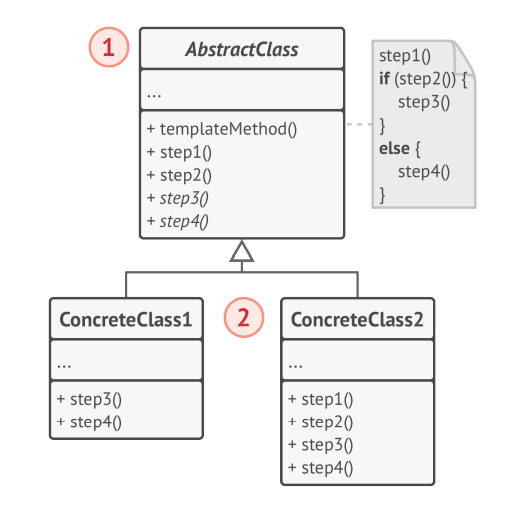
\includegraphics[scale=0.6]{image/behavioral/template.png}
\end{center}
\subsubsection{Ưu điểm và Nhược điểm}
Ta có rất nhiều ưu nhược điểm như sau:\\\\
Ưu điểm:
\begin{itemize}
    \item Các lớp con có thể thay đổi hoặc mở rộng các bước cụ thể của thuật toán mà không ảnh hưởng đến cấu trúc chung.
    \item  Mỗi bước của thuật toán được triển khai trong một phương thức riêng biệt, giúp tách rời và quản lý từng bước một.
    \item Cho phép người dùng override chỉ một số phần nhất định của thuật toán lớn, làm cho chúng ít bị ảnh hưởng hơn bởi những thay đổi xảy ra với các phần khác của thuật toán.
\end{itemize}
Nhược điểm:
\begin{itemize}
    \item Template method có càng nhiều bước để override càng khó bảo trì.
    \item Cần hiểu rõ khung (template) và cách các bước cụ thể được triển khai trong các lớp con.
\end{itemize}
\subsubsection{Code Example}
\begin{lstlisting}
#include <iostream>

// Abstract class defining the template method
class AbstractClass {
public:
    // Template method defining the algorithm
    void templateMethod() {
        step1();
        step2();
        step3();
    }

protected:
    virtual void step1() = 0;
    virtual void step2() = 0;
    virtual void step3() = 0;
};

// Concrete class implementing the template method
class ConcreteClass : public AbstractClass {
protected:
    void step1() override {
        std::cout << "ConcreteClass: Step 1" << std::endl;
    }

    void step2() override {
        std::cout << "ConcreteClass: Step 2" << std::endl;
    }

    void step3() override {
        std::cout << "ConcreteClass: Step 3" << std::endl;
    }
};

int main() {
    AbstractClass* abstractClass = new ConcreteClass();
    abstractClass->templateMethod();

    delete abstractClass;

    return 0;
}

\end{lstlisting}
Kết quả:
\begin{lstlisting}
ConcreteClass: Step 1
ConcreteClass: Step 2
ConcreteClass: Step 3
\end{lstlisting}
\subsubsection{Các Pattern liên quan}
\begin{itemize}
    \item Factory Method có thể đóng vai trò như một bước trong Template method là cơ sở chuyên môn hóa của Template Method.
\end{itemize}
\subsection{Visitor}
\subsubsection{Định nghĩa}
Visitor (Người ghé thăm) là một mẫu thiết kế hành vi cho phép thực hiện các thao tác trên các đối tượng của một tập hợp các lớp khác nhau mà không làm thay đổi cấu trúc của chúng. Mẫu này cho phép bạn định nghĩa các thao tác mới mà không phải thay đổi các lớp đã tồn tại và tách rời logic của các thao tác khỏi cấu trúc của các đối tượng.
\subsubsection{Cách sử dụng}
Ta có thể sử dụng Visitor Pattern trong các trường hợp sau:
\begin{itemize}
    \item Sử dụng khi cần thực hiện thao tác trên tất cả các phần tử của cấu trúc đối tượng phức tạp.
    \item Sử dụng khi một hành vi chỉ có ý nghĩa trong một số lớp của hệ thống phân cấp lớp, nhưng không có ý nghĩa trong các lớp khác.
    \item Khi có nhiều thao tác khác nhau cần thực hiện trên các đối tượng, và không muốn thay đổi các lớp của chúng.
\end{itemize}
\subsubsection{Cấu trúc}
\begin{center}
    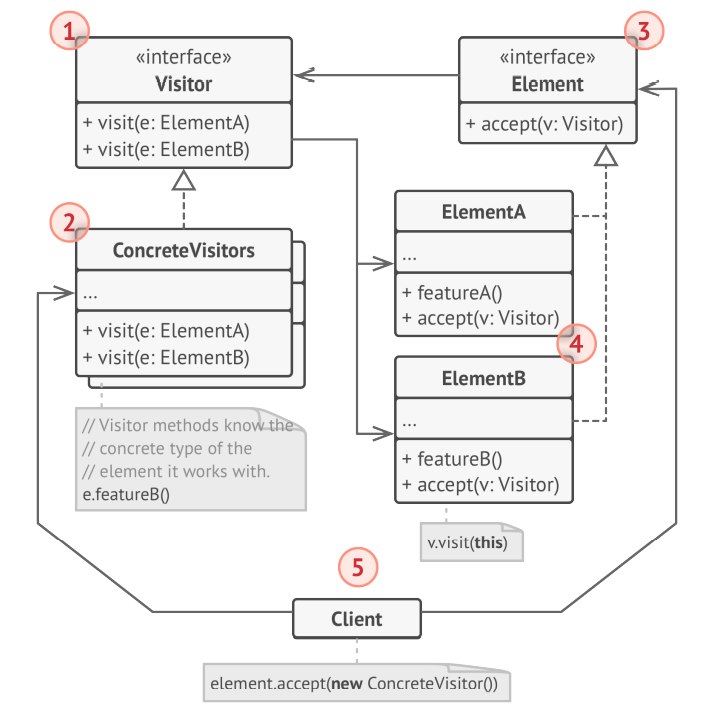
\includegraphics[scale=0.6]{image/behavioral/visitor.png}
\end{center}
\subsubsection{Ưu điểm và Nhược điểm}
Ta có rất nhiều ưu nhược điểm như sau:\\\\
Ưu điểm:
\begin{itemize}
    \item Một đối tượng visitor có thể tích lũy một số thông tin hữu ích khi làm việc với nhiều đối tượng khác nhau. Điều này có thể giúp ích khi ta muốn duyệt qua một số cấu trúc đối tượng phức tạp, chẳng hạn như cây đối tượng và áp dụng visitor cho từng đối tượng của cấu trúc này.
    \item Visitor cho phép tách rời logic của các thao tác khỏi cấu trúc của các đối tượng, giúp duy trì nguyên tắc đơn trách nhiệm (single responsibility principle).
    \item Visitor cho phép bạn thực hiện các thao tác khác nhau trên các đối tượng mà không cần thay đổi cấu trúc của chúng.
\end{itemize}
Nhược điểm:
\begin{itemize}
    \item Mẫu Visitor có thể làm tăng sự phức tạp của mã, đặc biệt khi có nhiều lớp và các thao tác phức tạp.
    \item Cần cập nhật tất cả visitor mỗi khi một lớp được thêm vào hoặc xóa khỏi hệ thống phân cấp phần tử.
    \item Các visitor có thể thiếu quyền truy cập cần thiết vào các trường riêng tư và phương thức của các phần tử mà họ phải làm việc với.
    \item Truyền đối tượng Visitor đến các đối tượng được ghé thăm có thể ảnh hưởng đến hiệu suất, đặc biệt khi có nhiều lớp và thao tác phức tạp.
\end{itemize}
\subsubsection{Code Example}
\begin{itemize}
    \item Có interface Element và 2 subclass.
    \item Có Abstract class Visitor và ConcreteVisitor.
\end{itemize}
\begin{lstlisting}
#include <iostream>
#include <vector>

// Forward declaration of classes
class ConcreteElementA;
class ConcreteElementB;

// Abstract Visitor class
class Visitor {
public:
    virtual void visit(ConcreteElementA* element) = 0;
    virtual void visit(ConcreteElementB* element) = 0;
};

// Abstract Element class
class Element {
public:
    virtual void accept(Visitor* visitor) = 0;
};

// Concrete Element A
class ConcreteElementA : public Element {
public:
    void accept(Visitor* visitor) override {
        visitor->visit(this);
    }

    std::string operationA() {
        return "ConcreteElementA";
    }
};

// Concrete Element B
class ConcreteElementB : public Element {
public:
    void accept(Visitor* visitor) override {
        visitor->visit(this);
    }

    std::string operationB() {
        return "ConcreteElementB";
    }
};

// Concrete Visitor
class ConcreteVisitor : public Visitor {
public:
    void visit(ConcreteElementA* element) override {
        std::cout << "ConcreteVisitor: Visit " << element->operationA() << std::endl;
    }

    void visit(ConcreteElementB* element) override {
        std::cout << "ConcreteVisitor: Visit " << element->operationB() << std::endl;
    }
};

int main() {
    // Create elements
    ConcreteElementA elementA;
    ConcreteElementB elementB;

    // Create visitor
    ConcreteVisitor visitor;

    // Accept visitor on elements
    elementA.accept(&visitor);
    elementB.accept(&visitor);

    return 0;
}

\end{lstlisting}
Ở hàm main, tạo ra 2 elements và một visitor cơ bản. Sau đó ta cho 2 elements này chấp nhận Visitor và cho ra kết quả.\\
\newline
\textbf{Kết quả:}
\begin{lstlisting}
ConcreteVisitor: Visit ConcreteElementA
ConcreteVisitor: Visit ConcreteElementB
\end{lstlisting}
\subsubsection{Các Pattern liên quan}
\begin{itemize}
    \item Một phiên bản hiệu quả của Command.
    \item Dùng Visitor để thực hiện thao tác trên cây Composite.
    \item Kết hợp với Iterator để duyệt qua cấu trúc dữ liệu phức tạp và thực hiện một vài Operation trên các phần tử của nó.
\end{itemize}
\newpage
\section{Lời kết}
\begin{itemize}
    \item Khi chúng ta khám phá và áp dụng Design Pattern, chúng ta mở ra cánh cửa của một thế giới bất tận của kiến thức và công nghệ. Design Pattern không chỉ là một bộ công cụ giúp chúng ta giải quyết các vấn đề trong thiết kế phần mềm, mà nó còn là một nguồn cảm hứng, một hướng dẫn và một ngôn ngữ chung giữa các nhà phát triển.
    \item Qua việc áp dụng Design Pattern, chúng ta học cách tách rời và tái sử dụng các thành phần, tăng tính linh hoạt và dễ bảo trì của hệ thống. Chúng ta học cách xây dựng các kiến trúc mạnh mẽ, đảm bảo tính mở rộng và khả năng mở rộng trong tương lai.
    \item Tuy nhiên, cần lưu ý rằng Design Pattern không phải là một giải pháp tuyệt đối cho mọi vấn đề trong phát triển phần mềm. Chúng ta cần hiểu rõ bản chất của vấn đề và chọn lựa Design Pattern phù hợp để áp dụng. Đôi khi, việc quá sử dụng Design Pattern có thể làm cho hệ thống phức tạp hơn và khó hiểu hơn.
    \item Điều quan trọng nhất khi sử dụng Design Pattern là hiểu rõ mục đích và nguyên tắc đằng sau nó. Design Pattern không chỉ là một mô hình mã lệnh cụ thể, mà là một khái niệm thiết kế, một tư duy để giúp chúng ta đưa ra các quyết định thông minh và linh hoạt.
    \item Cuối cùng, việc học và áp dụng Design Pattern đòi hỏi thời gian và kỷ luật. Hãy sử dụng Design Pattern như một công cụ hỗ trợ, không phải là một rào cản trong quá trình phát triển phần mềm. Với sự am hiểu và sử dụng đúng cách, Design Pattern sẽ là một người bạn đồng hành đáng tin cậy trên con đường xây dựng phần mềm chất lượng cao.
\end{itemize}
\newpage
\section{Tài liệu tham khảo}
Trong quá trình làm bài, có một số tài liệu tham khảo được sử dụng:\\
\url{https://viblo.asia/p/tong-hop-cac-bai-huong-dan-ve-design-pattern-23-mau-co-ban-cua-gof-3P0lPQPG5ox}
\url{https://refactoring.guru/design-patterns}
\url{https://topdev.vn/blog/design-pattern-la-gi/}
\url{https://itviec.com/blog/design-pattern/}
\url{https://bagps.vn/public/media/cv/0962543321_cv.pdf}
\url{https://www.amazon.com/Design-Patterns-Object-Oriented-Addison-Wesley-Professional-ebook/dp/B000SEIBB8}

\printbibliography[heading=bibintoc]

\end{document}
